\chapter{Muon Interaction} \label{sec:interactions}

The muon cross-sections described in this chapter focus on muons above a GeV and the relevant processes for the simulation of astroparticle experiments.
These processes are all included in the simulation library PROPOSAL or are intended to be included in the future.
In principle, they are also valid for the other charged leptons, electrons, and taus, if not stated differently.
% At least at high energies the deviations due to interferences or the different mass vanishes.

All cross-sections $\sigma$ are differential in the energy loss $v$ relative to the energy of the primary particle $E$, given as $\dif \sigma / \dif v$ or as the average energy loss over distance $X$
\begin{align} \label{eq:dedx_int}
    \left\langle - \frac{\dif E}{\dif X} \right\rangle = \frac{N_A}{A} E \int v \frac{\dif \sigma}{\dif v} \dif v.
\end{align}
The cross-sections are also given in a generalized form for particles with mass $M$ and charge $z$.
Mainly the natural unit system is used with the symbolic definitions listed in \tabref{tab:symbols}.
\begin{table}
    \centering
    \caption{Definitions of the symbols used in this thesis, unless stated otherwise or mentioned explicitly.}
    \label{tab:symbols}
    \begin{tabular}{cl}
        \toprule
        Symbol & Definition \\
        \midrule
        $c_0$ & Speed of light in vacuum ($=1$ in n.u. and $\approx \SI{3e8}{m.\per.s}$ in SI units) \\
        $N_A$ & Avogadro constant ($\approx \SI{6e23}{\per.\mol}$) \\
        $\alpha$ & Fine structure constant ($\approx 1/137$) \\
        $m_{e,\mu,\dots}$ & Mass of a particle with the lower index defining the particle type \\
        $r_{e (\mu)}$ & Classical electron (muon) radius ($r_e\approx \SI{2.8}{fm}, r_\mu = r_e \sfrac{m_e}{m_\mu}$) \\
        $E, p$ & Energy and momentum of a particle with $E^2 = p^2 + m^2$\\
        $\beta$, $\gamma$ & Lorentz factors in relativistic approximation, $\beta = p/E$ and  $\gamma = E/m$ \\
        $M, z$ & Mass and charge of the primary particle to propagate \\
        $Z, A$ & Number of protons (nucleons) in the target nucleus \\
        $K$ & Ionization constant $4\pi N_A r_e^2 m_e \approx \SI{0.3}{MeV.cm^2 / mol}$ \\
        $X_0$ & Radiation length of a medium (c.f. \ref{sec:medium}) \\
        $q, Q^2$ & 4-momentum of the virtual photon exchanged with a nucleus \\
        $B_{\text{(in)el}}$ & (in)elastic radiation logarithm constant of the screening (section \ref{sec:medium}) \\
        \bottomrule
    \end{tabular}
\end{table}

An overview of the energy loss of muons is shown in \figref{fig:dedx_pdg} which is divided into four areas in energy.
At the lowest energies ($\beta < \alpha$) the velocity of the muons is smaller than the velocity of the valence electrons.
Non-ionizing losses mainly driven by nuclear recoil are the main process for $\beta \ll \alpha$ before ionizing energy losses increase proportionally to the velocity of the muon \cite{Groom01}.
The energy region between $\alpha < \beta < \num{0.1}$ is not yet theoretically well understood and only empirical models are used to describe these energy losses \cite{Groom01}.
For both low energy regions, the data in \figref{fig:dedx_pdg} are taken from pion and proton tables in \cite{ICRU49} and scaled according to the mass ratios to the muon.
Both regions also differ between $\mu^+$ and $\mu^-$ since the latter is likely to get captured into atomic orbitals, quickly cascading down into the 1s orbital and then decay or weakly interact with the nucleus (c.f. \cite{Measday01}).

For $\beta > \num{0.1}$, the ionization and excitation losses are well described by the Bethe-Bloch theory.
The energy loss decreases to a minimum ionization point, a characteristic energy for a medium at around a GeV before it starts increasing logarithmically with the energy.
The radiative losses, i.e. bremsstrahlung, pair production, and inelastic nuclear interaction, increase linearly with the energy surpassing the ionization losses at a TeV and dominating the energy loss at high energies.
Initially, the inelastic nuclear interaction is just a \SI{10}{\%} correction compared to the other two processes, but increases slightly quicker and surpassing the other two even before the LPM-effect limits them, which occur between PeV and ZeV energies and is therefore not included in \figref{fig:dedx_pdg}.
\begin{figure}
    \centering
    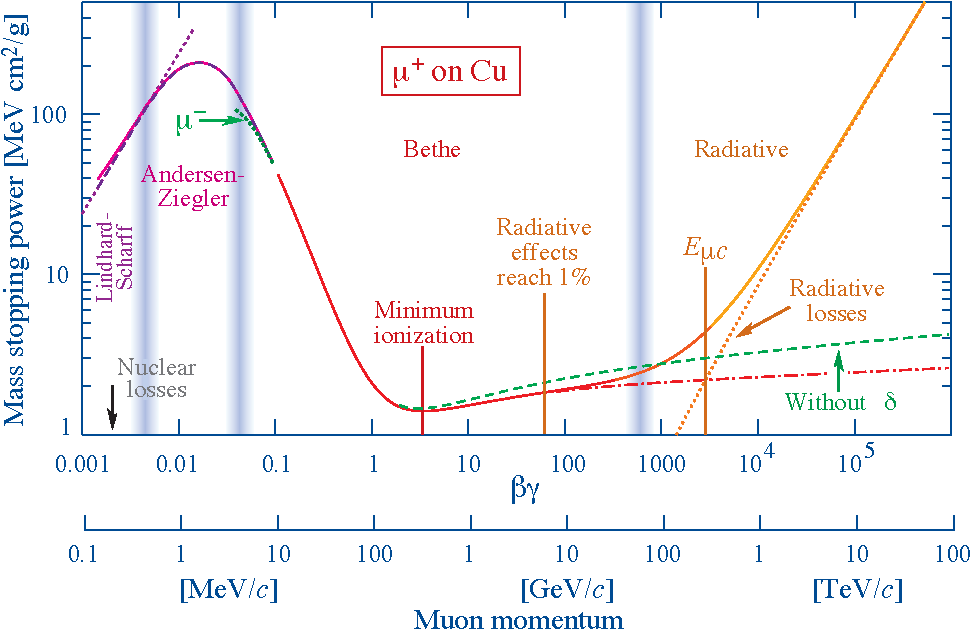
\includegraphics[width=0.82\textwidth]{./images/muon_dedx_pdg.pdf}
    \caption{Average energy loss of muons in copper. \cite{PDG20}}
    \label{fig:dedx_pdg}
\end{figure}

%
% new section
%

\section{The average Energy Loss} \label{sec:dedx}

At energies above a GeV, muons lose their energy via four main interaction types, ionization, $e^+e^-$ pair production, bremsstrahlung, and inelastic nuclear interactions, which is often referred to as photonuclear interaction.
While the ionization is nearly constant and just increases logarithmically with the energy, the other three processes increase linearly with the energy surpassing the Ionization at around a TeV, depending on the medium.
This behavior can be visualized in the average energy loss in \figref{fig:dedx_pdg}.
Besides the four main interactions, there are further processes with just minor influence on the energy loss, but also important for the muon propagation, the $\mu^+\mu^-$ pair production, and the weak interaction.
Regarding the decay, the muons have a relatively long lifetime of around \SI{2.2}{\micro\second} \cite{PDG20}.
They usually lose nearly all of their energy, slow down that the $\mu^-$ even get absorbed by an atom and decay with a total energy of almost their rest mass.
Therefore, the decay process does also not contribute to the energy loss as indicated in \figref{fig:dedx_all}.

As the weak interaction and the decay are purely stochastic processes and have no continuous energy loss, their contribution in \figref{fig:dedx_all} is adapted.
For both the decay and the weak interaction, the average energy loss is indicated by multiplying the energy times the total cross-section.
Using the mean lifetime $\tau$, the cross-section for the decay is defined by
\begin{align} \label{eq:sigma_decay}
    \sigma_{\text{decay}} = \frac{1}{\beta \gamma \tau c_0}.
\end{align}
The sum of the energy loss can be parameterized using a quasi-linear approximation
\begin{align} \label{eq:dedx_approx}
    \left\langle - \frac{\dif E}{\dif X} \right\rangle = a(E) + b(E) \cdot E.
\end{align}
Thereby, the functions $a$ and $b$ only depend logarithmically on the energy, while $a$ is mainly defined by the Ionization and $b$ by the three radiative processes.

Assuming $a$ and $b$ as constant values, the average range of the muons can be approximated by
\begin{align} \label{eq:dedx_range}
    R_{\left\langle -\frac{\dif E}{\dif X} \right\rangle} = \frac{1}{b} \logn \left( 1 + \frac{b}{a} E \right).
\end{align}
This simple linear model, shown in \figref{fig:dedx_range}, already provides a rough description of the muon energy loss and range and is used in many applications as a first estimation of the muon contribution.
A comparison with more precise calculations of the range using Monte-Carlo techniques is shown in \figref{fig:prop_range}.
\begin{figure}
    \centering
    \begin{subfigure}{0.9\textwidth}
        \centering
        \includegraphics[width=\textwidth]{./plots/dedx_all.pdf}
        \caption{The average energy loss of muons.}
        \label{fig:dedx_all}
        \vspace{0.5cm}
    \end{subfigure}
    \begin{subfigure}{0.9\textwidth}
        \centering
        \includegraphics[width=\textwidth]{./plots/dedx_range.pdf}
        \caption{The average range of muons using the $\left\langle -\frac{\dif E}{\dif X} \right\rangle$ fit.}
        \label{fig:dedx_range}
    \end{subfigure}
    \caption{The average energy loss and range of muons in Standard Rock ($Z=11, A=22$) using the linear approximation in \ref{eq:dedx_approx}. The fitted values are then used to calculate the average range given by \ref{eq:dedx_range}. The contribution of the decay and the weak interaction to the \enquote{continuous energy loss} is described in the text.}
    \label{fig:dedx}
\end{figure}

%
% new section
%

\section{Ionization} \label{sec:ioniz}

The ionization describes the release of an electron from the atomic shell, producing an ion.
Regarding the muon cross-sections, the excitation of an atom and the scattering at atomic electrons are included in the wider meaning of Ionization.
In contrast to all other interactions, the ionization is given as differential cross-section, but also in the average energy loss, since the density effect can only be included in the average energy loss.

The differential cross-section describing the knock-on electrons was mainly derived by Bethe \cite{Bethe30} and combined with further corrections into an expression by Rossi \cite{Rossi52}.
\begin{align} \label{eq:ioniz_dsigma}
\frac{\dif \sigma}{\dif v} = 
    \frac{1}{2} K z^2 \frac{Z}{A} \frac{1}{(\beta Ev)^2}
    \left[ 1 - \beta^2 \frac{v}{v_{\text{max}}} + \frac{1}{2} \left( \frac{v}{1 + 1/\gamma} \right)^2
    \right]
\end{align}
The $1/v^2$ dependency already indicates that this cross-section is responsible for the lower energy losses.
The maximum energy transferred to the electrons is given by \cite{PDG20}
\begin{align} \label{eq:ioniz_vmax}
    E v_{\text{max}} = \frac{2 m_e \beta^2 \gamma^2}{1 + 2 \gamma \frac{m_e}{M} + \left(\frac{m_e}{M}\right)^2},
\end{align}
which is an analytic interpolation between the approximations of the extreme scenarios at low and high energies
\begin{align}
    Ev_{\text{max}} =
    \begin{cases} 
        2m_e\beta^2 \gamma^2, & \text{ for } 2\gamma m_e \ll M \\
        M \beta^2 \gamma & \text{ for } 2\gamma m_e \gg M.
    \end{cases}
\end{align}
According to \eqref{eq:dedx_int} the average energy loss is obtained by integrating \eqref{eq:ioniz_dsigma} between
\begin{align}
    v_{\text{min}} = \frac{1}{2m_eE} \left( \frac{I_{\text{excit.}}}{\beta\gamma} \right)^2,
\end{align}
and a $v_{\text{up}}$ located between the limits.
Including the correction of the density effect $\delta$, this results in
\begin{align}
\frac{\dif E}{\dif X} = z^2 \frac{Z}{A} \frac{K}{2\beta^2}
    \left[
        \logn \frac{2 m_e \beta^2 \gamma^2 Ev_{\text{up}}}{I_{\text{excit.}}^2}
        - \beta^2 \left( 1 + \frac{v_{\text{up}}}{v_{\text{max}}} \right)
        + \left( \frac{v_\text{up}}{2(1 + 1/\gamma)} \right)^2
        - \delta
    \right]
\end{align}
with $I_{\text{excit.}}$ the mean excitation energy of the medium.
The reason for integrating to $v_{\text{up}}$ instead of $v_{\text{max}}$ is due to the energy loss cut, described in section \ref{sec:ecuts}, that is necessary for the simulations.

The density effect describes the reduction of the ionization due to the polarisation of the medium, which has an increasing effect at higher energies, indicated in \figref{fig:dedx_pdg}.
This is not included in the differential cross-section as it is a purely continuous energy loss process and not a stochastic interaction.
Depending on the energy parameter $x = \log_{10}(\beta\gamma)$, it is parameterized in \cite{Sternheimer52}
\begin{align}
\delta =
    \begin{cases}
        \delta_0 10^{2(x - x_0)}, & \text{ for } x < x_0\\
        2 \logn 10 x + c + a(x_1 - x)^b, & \text{ for } x_0 \leq x \leq x_1 \\
        2 \logn 10 x + c & \text{ for } x_1 \leq x
    \end{cases}
\end{align}
The density constants $\delta_0, x_0, x_1, a, b, c$ as well as the excitation energy $I_{\text{excit.}}$ are specific constants for each medium and defined in \cite{Groom01}.
For selected media that are implemented in PROPOSAl, these constants are listed in \tabref{tab:ioniz_const}.
\begin{table}
    \caption{The excitation energy and further density correction parameters for selected media mainly used in PROPOSAL. \cite{Groom01}}
    \label{tab:ioniz_const}
    \begin{center}
    \begin{tabular}{l | S[table-format=3.1] S[table-format=+1.4] S[table-format=1.4] S[table-format=1.5] S[table-format=1.4] S[table-format=2.4] S[table-format=1.2]}
        \toprule
        Medium & {$I_{\text{excit.}}$} & {$x_0$} & {$x_1$} & {$a$} & {$b$} & {$-c$} & {$\delta_0$} \\
        \midrule
        Air           & 85.7  & 1.7418 & 4.2759 & 0.10914 & 3.3994 & 10.5961 & 0 \\
        Water         & 79.7  & 0.2400 & 2.9004 & 0.09116 & 3.4773 & 3.5017 & 0 \\
        Ice           & 79.7  & 0.2586 & 2.8190 & 0.09116 & 3.4773 & 3.5873 & 0 \\
        Standard Rock & 136.4 & 0.0492 & 3.0549 & 0.08301 & 3.4120 & 3.7738 & 0 \\
        Iron          & 286.0 & -0.0012 & 3.1531 & 0.14680 & 2.9632 & 4.2911 & 0.12 \\
        Uranium       & 890.0 & 0.2260 & 3.3721 & 0.19677 & 2.8171 & 5.8694 & 0.14 \\
        \bottomrule
    \end{tabular}
    \end{center}
\end{table}

The inelastic bremsstrahlung on atomic electrons when the atomic electron emits the bremsstrahlung, described in section \ref{sec:brems_inel}, is most often considered as an ionization loss since the atom also gets ionized.
While the main bremsstrahlung cross-section has an energy loss behavior of $1/v$ the so-called $e$-diagrams (see the Feynman diagram in \figref{fig:feyn_brems_e}) have a sharp energy loss spectrum of $1/v^2$, shown in \eqref{eq:brems_e_diagram}, similar to ionization.

The differential cross section of the ionization processes is shown in \figref{fig:ioniz_dsigma} mainly showing the $1/v^2$ dependency and a flattening of the $e$-diagram bremsstrahlung to small energy losses due to the parametrization.
In \figref{fig:ioniz_dedx} the average energy loss of the two contributions and the additional density correction are shown.
\begin{figure}
    \centering
    \begin{subfigure}{0.9\textwidth}
        \centering
        \includegraphics[width=\textwidth]{./plots/ioniz_dsigma.pdf}
        \caption{The differential cross section of the ionization processes at \SI{1}{TeV}.}
        \label{fig:ioniz_dsigma}
        \vspace{0.5cm}
    \end{subfigure}
    \begin{subfigure}{0.9\textwidth}
        \centering
        \includegraphics[width=\textwidth]{./plots/ioniz_dedx.pdf}
        \caption{The average energy loss of the ionization processes.}
        \label{fig:ioniz_dedx}
    \end{subfigure}
    \caption{The Ionization cross-section of muons in Standard Rock ($Z=11, A=22$). The Bethe-Bloch term is compared to the inelastic interaction on atomic electrons with the electrons emitting a bremsstrahlung photon ($e$-diagram) and the negative contribution of the density correction.}
    \label{fig:ioniz}
\end{figure}

%
% new section
%

\section{Bremsstrahlung} \label{sec:brems}

The Bremsstrahlung process, where the muon emits a photon and exchanges the remaining momentum with a nucleus in an elastic process, can be visualized in the Feynman diagrams in \figref{fig:feyn_brems}.
\begin{figure}
    \centering
    %
\begin{tikzpicture}
\begin{feynman}
    % define vertices
    % muon
    \vertex (mu_in) at (-\feynlen-\feynsmallen, 0);
    \vertex[right=2.5*\feynlen of mu_in] (mu_out);
    \vertex[right=\feynlen of mu_in] (mu_vertex_nucl);
    \vertex[left=\feynlen of mu_out] (mu_vertex_brems);
    % brems
    \vertex[above=\feynlen of mu_out] (brems_out);
    % nucleus
    \vertex[below=\feynlen of mu_in] (n_in);
    \vertex[below=\feynlen of mu_vertex_nucl] (n_vertex);
    \vertex[below=\feynlen of mu_out] (n_out);
    % draw diagram
    \diagram* {
        (mu_in) -- [fermion] (mu_vertex_nucl) -- (mu_vertex_brems) -- [fermion] (mu_out),
        (mu_vertex_nucl) -- [boson] (n_vertex),
        (mu_vertex_brems) -- [boson] (brems_out)
    };
    % draw extra features with tikz (not available in tikz-feynman)
    \draw[thick, double] (n_in) -- (n_vertex) -- (n_out);
    \draw[fill] (n_vertex) circle[radius=\feynvertexsize];
    \draw[fill] (mu_vertex_nucl) circle[radius=\feynvertexsize];
    \draw[fill] (mu_vertex_brems) circle[radius=\feynvertexsize];
    % add labels
    \node[left] at (mu_in) {$\mu$};
    \node[right] at (mu_out) {$\mu '$};
    \node[right] at (brems_out) {$\gamma$};
    \node[left] at (n_in) {$N$};
    \node[right] at (n_out) {$N'$};
\end{feynman}
\end{tikzpicture}
%
\hspace{1cm}
%
\begin{tikzpicture}
\begin{feynman}
    % define vertices
    % muon
    \vertex (mu_in) at (-\feynlen-\feynsmallen, 0);
    \vertex[right=2.5*\feynlen of mu_in] (mu_out);
    \vertex[left=\feynlen of mu_out] (mu_vertex_nucl);
    \vertex[right=\feynlen of mu_in] (mu_vertex_brems);
    % brems
    \vertex[above=\feynlen of mu_out] (brems_out);
    % nucleus
    \vertex[below=\feynlen of mu_in] (n_in);
    \vertex[below=\feynlen of mu_vertex_nucl] (n_vertex);
    \vertex[below=\feynlen of mu_out] (n_out);
    % draw diagram
    \diagram* {
        (mu_in) -- [fermion] (mu_vertex_brems) -- (mu_vertex_nucl) -- [fermion] (mu_out),
        (mu_vertex_nucl) -- [boson] (n_vertex),
        (mu_vertex_brems) -- [boson] (brems_out)
    };
    % draw extra features with tikz (not available in tikz-feynman)
    \draw[thick, double] (n_in) -- (n_vertex) -- (n_out);
    \draw[fill] (n_vertex) circle[radius=\feynvertexsize];
    \draw[fill] (mu_vertex_nucl) circle[radius=\feynvertexsize];
    \draw[fill] (mu_vertex_brems) circle[radius=\feynvertexsize];
    % add labels
    \node[left] at (mu_in) {$\mu$};
    \node[right] at (mu_out) {$\mu '$};
    \node[right] at (brems_out) {$\gamma$};
    \node[left] at (n_in) {$N$};
    \node[right] at (n_out) {$N'$};
\end{feynman}
\end{tikzpicture}
%
    \caption{The two Feynman diagrams of a muon emitting a Bremsstrahlung photon and exchange a momentum with a nucleus are shown, differing in the order when the photon to the nucleus and the bremsstrahlung photon couples to the muon line.}
    \label{fig:feyn_brems}
\end{figure}

A general expression of the cross-section was first derived in \cite{Bethe34}
\begin{align} \label{eq:brems}
\frac{\dif \sigma}{\dif v} =
    \frac{\alpha}{v} \left(2z^2Z r_e \frac{m_e}{M}\right)^2
    \left[ (2 - 2v + v^2) \Phi_1 - \frac{2}{3} (1 - v) \Phi_2 \right],
\end{align}
with the screening functions $\Phi_1$ and $\Phi_2$ described later.
The two main behaviors of the cross-section can already be seen here.
First, the mass ratio $m_e / M$ explains, why bremsstrahlung is the dominating process of high energetic electrons, that it is still significant for muons and negligible for heavier particles like taus.
Second, the flat $1/v$ dependency is responsible for the large stochasticity of the bremsstrahlung interaction since on a logarithmic scale the probability for a small continuous loss is equal to that of a large stochastic loss.

Due to the $1/v$ dependence of the differential cross-section, there is a divergence for small energy losses due to the massless photon, which can be interpreted as an infinite probability to emit a photon with no energy.
Although the average energy loss is finite, this is a problem for numerical simulations.
In Monte-Carlo simulations, this issue is solved by splitting the calculation of the interaction probabilities into a continuous and stochastic propagation, described in section \ref{sec:simulation}.

The limits on the energy loss for the bremsstrahlung cross-section are
\begin{align}
    v_{\text{min}} = 0
    \quad
    \text{ and }
    \quad
    v_{\text{max}} = 1 - \frac{3}{4}\frac{M}{E}\sqrt{e}Z^{\sfrac13}.
\end{align}
While the lower bound for the energy loss is set by the massless photon, the upper bound is in principle just limited by the particle mass $1-M/E$.
However, the part of the Feynman diagram describing the nuclear interaction is just described effectively using approximations.
The upper bound is defined by the logarithms in the screening functions, described in section \ref{sec:brems_screen}, so the resulting cross-section does not become negative, which would be unphysical.
Therefore, the edge of the phase space where the muon loses all its energy to the photon is not described properly, yet.
For all calculations described in this section, the assumption of only relativistic particles is used i.e. $M \ll E$.
\begin{figure}[H]
    \centering
    \includegraphics[width=0.8\textwidth]{./plots/brems_contributions.pdf}
    \caption{Differential cross-section of the muon bremsstrahlung at an energy of \SI{1}{TeV} in Standard Rock ($Z=11, A=22$).}
    \label{fig:brems_dsigma}
\end{figure}

The differential cross-section is shown in \figref{fig:brems_dsigma} mainly illustrating the $1/v$ dependency and the relevant processes influencing the cross-section.
The following subsections describe these effects contributing including the elastic and inelastic nuclear and atomic form factor as well as the coulomb and radiation correction and finally the matter effects.
All these processes do also appear for the pair production processes.
To not duplicate the passages, these effects are mainly described in this section.

\subsection{Screening Functions for elastic Interactions} \label{sec:brems_screen}

The simplest way to describe the nuclear interaction is using a coulomb field of a point-like particle with the charge $Z$.
However, a more advanced approach describes the nucleus of a finite size which is surrounded and screened by atomic electrons.
The Fourier transform of the radial charge distribution of the nucleus, called the \textit{nuclear form factor}, is used to include these effects in the screening functions.
For the atomic electrons, the corresponding Fourier transform is called the \textit{atomic form factor}.
These functions only depend on the minimum momentum transfer to the nucleus given by
\begin{align}
    \delta = \frac{M^2 v}{2E(1 - v)}.
\end{align}
Since the form factors effect different regions of $Q^2$, the screening functions can be separated into a part $\Phi^0$ at low $Q^2$ where the atomic form factor dominates and a part $\Delta$ at high $Q^2$ where the nuclear form factor dominates
\begin{align} \label{eq:screen}
    \Phi = \begin{cases}
        \Phi^0 - \Delta, & Z=1 \\
        \Phi^0 - \Delta(1 - \frac{1}{Z}) & Z>1.
    \end{cases}
\end{align}
Assuming a point-like nucleus the screening functions can be described in the extreme cases of no screening (ns) and full screening (fs) by
\begin{subequations} \label{eq:brems_ns_fs}
\begin{align}
    \Phi_{1, \mathrm{ns}}^0 &= \logn \frac{M}{\delta} - \frac{1}{2}
    & \Phi_{2, \mathrm{ns}}^0 &= \Phi_1^0
    \\
    \Phi_{1, \mathrm{fs}}^0 &= \logn \left( \frac{M}{m_e} B_{\text{el}} Z^{-\sfrac13} \right)
    & \Phi_{2, \mathrm{fs}}^0 &= \Phi_1^0 - \frac{1}{6}
\end{align}
\end{subequations}
An analytical interpolation between these extreme scenarios have been calculated in \cite{Sandrock18PhD} using the techniques of \cite{Petrukhin68} resulting in 
\begin{align} \label{eq:brems_screen_interpol}
    \Phi_1^0 =
        \logn \frac{\frac{M}{m_e} B_{\text{el}}Z^{-\sfrac13}}{1 + \frac{\delta}{m_e}\sqrt{e} B_{\text{el}} Z^{-\sfrac13}}
    \quad
    \text{ and }
    \quad
    \Phi_2^0 =
        \logn \frac{\frac{M}{m_e} e^{-\sfrac16} B_{\text{el}}Z^{-\sfrac13}}{1 + \frac{\delta}{m_e} e^{\sfrac13} B_{\text{el}} Z^{-\sfrac13}}.
\end{align}
The interpolated screening together with the extreme scenarios are shown in \figref{fig:brems_dsigma} illustrating the relevance of the full screening for small energy losses and the transition to no screening at high energy losses.

For the nuclear form factor a step function can be used according to \cite{Bugaev77}, or more accurate parametrizations like a Fermi distribution, with the step at the critical momentum \cite{Kelner95Brems}
\begin{align}
    q_c = \frac{m_{\mu}e}{D_n}
    \qquad \text{with} \qquad
    D_n = 1.54 A^{0.27} .
\end{align}
The correction due to the finite size of the nucleus, decreasing the screening by around $\SI{10}{\percent}$, can be parametrized independent of $\delta$ by \cite{Andreev94Brems}
\begin{align}
    \Delta_1 = \logn \frac{M}{q_c} + \frac{\rho}{2} \logn \frac{\rho + 1}{\rho - 1}
    \quad
    \text{ and }
    \quad
    \Delta_2 = \logn \frac{M}{q_c} + \frac{3\rho - \rho^3}{4} \logn \frac{\rho + 1}{\rho - 1} + \frac{2 M^2}{q_c^2}
\end{align}
with $\rho = \sqrt{1 + \frac{4M^2}{q_c^2}}$.
This description of the nuclear form factor was calculated regarding muons, especially the fit for $D_n$.
In $q_c$ the muon mass is used explicitly, since $\hbar c_0 / m_\mu \approx \SI{2}{fm}$ is an axcellent scaling for nuclear sizes.
However, since the influence of the mass of the primary particle is just a small correction to an overall percent contribution, this is also applicable to particles with different mass, like electrons or taus.

The independence of the minimum momentum transfer only breaks at high values of $\delta$ near the muon mass.
Differences to calculations including this dependency \cite{Kelner95Brems} therefore only occur at high energy losses of $v \sim 1$ where the cross-section is already relatively small.
Since the general approximation of relativistic incoming and outgoing particles is assumed for all calculations presented here, the $\delta$ dependence is negligible.
In future parametrizations aiming to describe also the highest energy losses properly, this needs to be taken into account.

\subsection{Approximated Screening} \label{sec:brems_screen_approx}

Due to the small difference between the screening functions $\Phi_1$ and $\Phi_2$, which even vanishes in the no screening case, this difference is often neglected and the approximation
\begin{align} \label{eq:screen_approx}
    \Phi = \Phi_1 \approx \Phi_2
\end{align}
is used.
Thereby, the differential cross-section of \eqref{eq:brems} simplifies to
\begin{align} \label{eq:brems_approx}
\frac{\dif \sigma}{\dif v} =
    \frac{\alpha}{v} Z \left(2z r_e \frac{m_e}{M}\right)^2
    \left( \frac{4}{3}(1 - v) + v^2 \right) \Phi .
\end{align}
Following the parametrization of \cite{Kelner95Brems}, the \enquote{interpolation} between the extreme scenarios of the screening in \eqref{eq:brems_ns_fs} can be described with the no screening case corrected by the screening of to the atomic form factor $\Delta_a$ and the nuclear form factor $\Delta_n$.
\begin{align}
    \Phi = \logn \frac{M}{\delta} - \frac12 - \Delta_a - \Delta_n .
\end{align}
Here, the correction due to the nuclear form factor was calculated including the dependency of $\delta$.
\begin{align}
	\Delta_a = \logn \left( 1 + \frac{1}{\delta \sqrt{e} B_{\text{el}} Z^{-\sfrac13} / m_e} \right)
    \quad
    \text{and}
    \quad
    \Delta_n = \logn \frac{D_n}{1 + \delta (D_n \sqrt{e} - 2) / M} .
\end{align}
The difference between the approximated screening of \cite{Kelner95Brems} and without the approximation \cite{Sandrock18PhD} in the differential cross-section is shown in \figref{fig:brems_dsigma}.
The maximum error of this approximation is less than a percent.

This parametrization is widely used in the literature and the default in PROPOSAL under the name \textit{KelnerKokoulinPetrukhin}.

\subsection{Inelastic Corrections} \label{sec:brems_inel}

So far only the elastic interactions with the target atom have been discussed.
The inelastic nuclear form factor, describing the excitation of the nucleus, is already included in \eqref{eq:screen} and differs compared to the elastic nuclear form factor only by a factor of $1/Z$ \cite{Andreev94Brems}.
This is not the case for Hydrogen since there are no nuclear excitations.

The inelastic atomic form factor describes the interaction with atomic electrons as the target particle that is screened by the field of the nucleus.
As shown in \figref{fig:feyn_brems_inel} it consists of two types of diagrams depending on whether the muon or the electron emits the bremsstrahlung photon.
\begin{figure}
    \begin{subfigure}{0.48\textwidth}
        \centering
        %
\begin{tikzpicture}
\begin{feynman}
    % define vertices
    % muon
    \vertex (mu_in) at (-\feynlen-\feynsmallen, 0);
    \vertex[right=2.5*\feynlen of mu_in] (mu_out);
    % brems
    \vertex[above=\feynlen of mu_out] (brems_out);
    % blob
    \vertex[right=1.25*\feynlen of mu_in] (blob);
    \vertex (blob_left) at ($(blob) + (180:\feynsmallen)$);
    \vertex (blob_right) at ($(blob) + (0:\feynsmallen)$);
    \vertex (blob_vertex) at ($(blob) + (-90:\feynsmallen)$);
    \vertex (blob_brems) at ($(blob) + (45:\feynsmallen)$);
    % nucleus/electron target
    \vertex[below=\feynlen of mu_in] (e_in);
    \vertex[below=\feynlen of mu_out] (e_out);
    \vertex[below=\feynlen of blob] (e_vertex);
    % draw diagram
    \diagram* {
        (mu_in) -- [fermion] (blob_left),
        (blob_right) -- [fermion] (mu_out),
        (e_in) -- [fermion] (e_vertex) -- [fermion] (e_out),
        (blob_vertex) -- [boson] (e_vertex),
        (blob_brems) -- [boson] (brems_out)
    };
    % draw extra features with tikz (not available in tikz-feynman)
    \draw[pattern = north east lines] (blob) circle[radius=\feynsmallen];
    \draw[fill] (e_vertex) circle[radius=\feynvertexsize];
    % add labels
    \node[left] at (mu_in) {$\mu$};
    \node[right] at (mu_out) {$\mu '$};
    \node[left] at (e_in) {$e$};
    \node[right] at (e_out) {$e'$};
    \node[right] at (brems_out) {$\gamma$};
\end{feynman}
\end{tikzpicture}
%
        \caption{$\mu$-diagram.}
        \label{fig:feyn_brems_mu}
    \end{subfigure}
    \hfill
    \begin{subfigure}{0.48\textwidth}
        \centering
        %
\begin{tikzpicture}
\begin{feynman}
    % define vertices
    % muon
    \vertex (mu_in) at (-\feynlen-\feynsmallen, \feynlen);
    \vertex[right=2.5*\feynlen of mu_in] (mu_out);
    \vertex[right=1.25*\feynlen of mu_in] (mu_vertex);
    % nucleus/electron target
    \vertex[below=\feynlen of mu_in] (e_in);
    \vertex[below=\feynlen of mu_out] (e_out);
    % brems
    \vertex[below=\feynlen of e_out] (brems_out);
    % blob
    \vertex[below=\feynlen of mu_vertex] (blob);
    \vertex (blob_left) at ($(blob) + (180:\feynsmallen)$);
    \vertex (blob_right) at ($(blob) + (0:\feynsmallen)$);
    \vertex (blob_vertex) at ($(blob) + (90:\feynsmallen)$);
    \vertex (blob_brems) at ($(blob) + (-45:\feynsmallen)$);
    % draw diagram
    \diagram* {
        (e_in) -- [fermion] (blob_left),
        (blob_right) -- [fermion] (e_out),
        (mu_in) -- [fermion] (mu_vertex) -- [fermion] (mu_out),
        (blob_vertex) -- [boson] (mu_vertex),
        (blob_brems) -- [boson] (brems_out)
    };
    % draw extra features with tikz (not available in tikz-feynman)
    \draw[pattern = north east lines] (blob) circle[radius=\feynsmallen];
    \draw[fill] (mu_vertex) circle[radius=\feynvertexsize];
    % add labels
    \node[left] at (mu_in) {$\mu$};
    \node[right] at (mu_out) {$\mu '$};
    \node[left] at (e_in) {$e$};
    \node[right] at (e_out) {$e'$};
    \node[right] at (brems_out) {$\gamma$};
\end{feynman}
\end{tikzpicture}
%
        \caption{$e$-diagram.}
        \label{fig:feyn_brems_e}
    \end{subfigure}
    \caption{The Feynman diagrams of the inelastic atomic form factors with the atomic electron as target. In the $\mu$-diagram the bremsstrahlung is emitted by the muon, in the $e$-diagram it is emitted by the electron. The patterned circles replace the two diagrams shown in \figref{fig:feyn_brems} differing in the order of the photons coupling to the fermion line.}
    \label{fig:feyn_brems_inel}
\end{figure}

The cross-section for the $\mu$-diagrams calculated in \cite{Kelner95Brems} is similar to \eqref{eq:brems_approx} also using the approximation $\Phi_1 \approx \Phi_2$.
The error due to this approximation does not increase the overall uncertainty since this contribution is already a correction to the main bremsstrahlung cross-section.
The screening function changes to $\Phi \to \Phi^{\text{inel}}$ with
\begin{align}
\Phi^{\text{inel}} =
    \logn \frac{M/\delta}{M\delta/m_e^2 + \sqrt{e}} - \logn \left( 1 + \frac{m_e}{\delta B_{\text{inel}}Z^{-\sfrac23}\sqrt{e}} \right) .
\end{align}
Due to the different target, the maximum energy loss, which is, in fact, the maximum energy that is transferred to the bremsstrahlung photon neglecting the energy transferred to the electron, changes to
\begin{align}
    v_{\text{max}} = \frac{m_e (E - M)}{E ( E - p + m_e)} .
\end{align}
As already mentioned in section \ref{sec:ioniz} the $e$-diagrams are considered with the ionization or knock-on electron process since the cross-section has a $1/v^2$ dependency and the average energy loss increases logarithmically with the energy.
The cross-section can be parametrized \cite{Kelner97Brems} as a correction factor to the ionization cross-section from \eqref{eq:ioniz_dsigma}.
\begin{align} \label{eq:brems_e_diagram}
\frac{\dif \sigma}{\dif v} =
    \frac{\dif \sigma}{\dif v}_{\text{ioniz}} \cdot
    \frac{\alpha}{2\pi} [ a(2b + c) - b^2 ]
\end{align}
with the logarithmic functions
\begin{align}
    a = \logn \left( 1 + \frac{2Ev}{m_e} \right), \quad
    b = \logn \frac{1 - v/v_{\text{max}}}{1 - v}
    \quad
    \text{ and }
    \quad
    c = \logn \frac{2 m_e \gamma (1-v)}{M v}.
\end{align}
The maximum energy loss here refers to the $v_{\text{max}}$ for the ionization in \eqref{eq:ioniz_vmax}.
The term $b$ is divergent for $v \to v_{\text{max}}$ which is an integrable singularity at the edge of the phase space but can causes issues in numerical calculations.
However, this is a minor correction to the main ionization term and only occurs at the highest energy losses where all other interactions dominate the ionization and can be neglected.
But it can still cause issues in numerical simulations and requires further investigations in upcoming works.

\subsection{Radiative Corrections} \label{sec:brems_nlo}

Reducing the uncertainty of the cross-section below the percent level also requires the inclusion of next-to-leading order (NLO) processes that are suppressed by a factor of $\alpha$ due to the additional vertex.
The diagrams for all NLO processes comprising vacuum polarization, self-energy, vertex correction, box diagram, and double bremsstrahlung are shown in \figref{fig:feyn_brems_nlo}.
\begin{figure}
    \begin{subfigure}[t]{0.3\textwidth}
        \centering
        %
\begin{tikzpicture}
\begin{feynman}
    % define vertices
    % muon
    \vertex (mu_in) at (-\feynlen, 0);
    \vertex[right=2.5*\feynlen of mu_in] (mu_out);
    \vertex[right=\feynlen of mu_in] (mu_vertex_nucl);
    \vertex[left=\feynlen of mu_out] (mu_vertex_brems);
    % brems
    \vertex[below=\feynlen of mu_out] (brems_out);
    % nucleus
    \vertex[below=2*\feynlen of mu_in] (n_in);
    \vertex[below=2*\feynlen of mu_vertex_nucl] (n_vertex);
    \vertex[below=2*\feynlen of mu_out] (n_out);
    % loop
    \vertex[below=\feynlen of mu_vertex_nucl] (loop);
    \vertex (loop_up) at ($(loop) + (90:\feynlen/3)$);
    \vertex (loop_down) at ($(loop) + (-90:\feynlen/3)$);
    % draw diagram
    \diagram* {
        (mu_in) -- [fermion] (mu_vertex_nucl) -- (mu_vertex_brems) -- [fermion] (mu_out),
        (mu_vertex_nucl) -- [boson] (loop_up),
        (n_vertex) -- [boson] (loop_down),
        (mu_vertex_brems) -- [boson] (brems_out),
        (loop_up) -- [fermion, half left] (loop_down) -- [fermion, half left] (loop_up)
    };
    % draw extra features with tikz (not available in tikz-feynman)
    \draw[thick, double] (n_in) -- (n_vertex) -- (n_out);
    \draw[fill] (n_vertex) circle[radius=\feynvertexsize];
    \draw[fill] (mu_vertex_nucl) circle[radius=\feynvertexsize];
    \draw[fill] (mu_vertex_brems) circle[radius=\feynvertexsize];
    \draw[fill] (loop_up) circle[radius=\feynvertexsize];
    \draw[fill] (loop_down) circle[radius=\feynvertexsize];
    % add labels
    \node[left] at (mu_in) {$\mu$};
    \node[right] at (mu_out) {$\mu '$};
    \node[right] at (brems_out) {$\gamma$};
    \node[left] at (n_in) {$N$};
    \node[right] at (n_out) {$N'$};
\end{feynman}
\end{tikzpicture}
%
        \caption{Vacuum Polarization.}
        \label{fig:feyn_brems_vacuum}
    \end{subfigure}
    \begin{subfigure}[t]{0.33\textwidth}
        \centering
        %
\begin{tikzpicture}
\begin{feynman}
    % define vertices
    % muon
    \vertex (mu_in) at (-\feynlen, 0);
    \vertex[right=3*\feynlen of mu_in] (mu_out);
    \vertex[right=0.85*\feynlen of mu_in] (mu_vertex_nucl);
    \vertex[left=0.85*\feynlen of mu_out] (mu_vertex_brems);
    % brems
    \vertex[below=0.75*\feynlen of mu_out] (brems_out);
    % nucleus
    \vertex[below=1.5*\feynlen of mu_in] (n_in);
    \vertex[below=1.5*\feynlen of mu_vertex_nucl] (n_vertex);
    \vertex[below=1.5*\feynlen of mu_out] (n_out);
    % loop
    \vertex[right=1.5*\feynlen of mu_in] (loop);
    \vertex (loop_left) at ($(loop) + (-180:\feynlen/3)$);
    \vertex (loop_right) at ($(loop) + (0:\feynlen/3)$);
    % draw diagram
    \diagram* {
        (mu_in) -- [fermion] (mu_vertex_nucl) -- (mu_vertex_brems) -- [fermion] (mu_out),
        (mu_vertex_nucl) -- [boson] (n_vertex),
        (loop_left) -- [boson, half left] (loop_right),
        (mu_vertex_brems) -- [boson] (brems_out)
    };
    % draw extra features with tikz (not available in tikz-feynman)
    \draw[thick, double] (n_in) -- (n_vertex) -- (n_out);
    \draw[fill] (n_vertex) circle[radius=\feynvertexsize];
    \draw[fill] (mu_vertex_nucl) circle[radius=\feynvertexsize];
    \draw[fill] (mu_vertex_brems) circle[radius=\feynvertexsize];
    \draw[fill] (loop_left) circle[radius=\feynvertexsize];
    \draw[fill] (loop_right) circle[radius=\feynvertexsize];
    % add labels
    \node[left] at (mu_in) {$\mu$};
    \node[right] at (mu_out) {$\mu '$};
    \node[right] at (brems_out) {$\gamma$};
    \node[left] at (n_in) {$N$};
    \node[right] at (n_out) {$N'$};
\end{feynman}
\end{tikzpicture}
%
        \caption{Self Energy.}
        \label{fig:feyn_brems_self}
    \end{subfigure}
    \begin{subfigure}[t]{0.33\textwidth}
        \centering
        %
\begin{tikzpicture}
\begin{feynman}
    % define vertices
    % muon
    \vertex (mu_in) at (-\feynlen, 0);
    \vertex[right=2.5*\feynlen of mu_in] (mu_out);
    \vertex[right=\feynlen of mu_in] (mu_vertex_nucl);
    \vertex[left=\feynlen of mu_out] (mu_vertex_brems);
    % brems
    \vertex[below=0.75*\feynlen of mu_out] (brems_out);
    % nucleus
    \vertex[below=1.5*\feynlen of mu_in] (n_in);
    \vertex[below=1.5*\feynlen of mu_vertex_nucl] (n_vertex);
    \vertex[below=1.5*\feynlen of mu_out] (n_out);
    % loop
    \vertex[right=1.25*\feynlen of mu_in] (loop);
    \vertex (loop_left) at ($(loop) + (-180:0.6*\feynlen)$);
    \vertex (loop_right) at ($(loop) + (0:0.6*\feynlen)$);
    % draw diagram
    \diagram* {
        (mu_in) -- [fermion] (loop_left) -- (loop_right) -- [fermion] (mu_out),
        (mu_vertex_nucl) -- [boson] (n_vertex),
        (loop_left) -- [boson, half left] (loop_right),
        (mu_vertex_brems) -- [boson] (brems_out)
    };
    % draw extra features with tikz (not available in tikz-feynman)
    \draw[thick, double] (n_in) -- (n_vertex) -- (n_out);
    \draw[fill] (n_vertex) circle[radius=\feynvertexsize];
    \draw[fill] (mu_vertex_nucl) circle[radius=\feynvertexsize];
    \draw[fill] (mu_vertex_brems) circle[radius=\feynvertexsize];
    \draw[fill] (loop_left) circle[radius=\feynvertexsize];
    \draw[fill] (loop_right) circle[radius=\feynvertexsize];
    % add labels
    \node[left] at (mu_in) {$\mu$};
    \node[right] at (mu_out) {$\mu '$};
    \node[right] at (brems_out) {$\gamma$};
    \node[left] at (n_in) {$N$};
    \node[right] at (n_out) {$N'$};
\end{feynman}
\end{tikzpicture}
%
        \caption{Box Diagram.}
        \label{fig:feyn_brems_box}
    \end{subfigure}
    \begin{subfigure}{0.96\textwidth}
        \vspace{0.5cm}
        \centering
        %
\begin{tikzpicture}
\begin{feynman}
    % define vertices
    % muon
    \vertex (mu_in) at (-\feynlen, 0);
    \vertex[right=3*\feynlen of mu_in] (mu_out);
    \vertex[right=0.85*\feynlen of mu_in] (mu_vertex_nucl);
    \vertex[left=1.25*\feynlen of mu_out] (mu_vertex_brems);
    % brems
    \vertex[below=0.75*\feynlen of mu_out] (brems_out);
    % nucleus
    \vertex[below=1.5*\feynlen of mu_in] (n_in);
    \vertex[below=1.5*\feynlen of mu_vertex_nucl] (n_vertex);
    \vertex[below=1.5*\feynlen of mu_out] (n_out);
    % loop
    \vertex (loop) at (mu_vertex_brems);
    \vertex (loop_left) at ($(loop) + (-180:0.45*\feynlen)$);
    \vertex (loop_right) at ($(loop) + (0:0.45*\feynlen)$);
    % draw diagram
    \diagram* {
        (mu_in) -- [fermion] (mu_vertex_nucl) -- (loop_right) -- [fermion] (mu_out),
        (mu_vertex_nucl) -- [boson] (n_vertex),
        (loop_left) -- [boson, half left] (loop_right),
        (mu_vertex_brems) -- [boson] (brems_out)
    };
    % draw extra features with tikz (not available in tikz-feynman)
    \draw[thick, double] (n_in) -- (n_vertex) -- (n_out);
    \draw[fill] (n_vertex) circle[radius=\feynvertexsize];
    \draw[fill] (mu_vertex_nucl) circle[radius=\feynvertexsize];
    \draw[fill] (mu_vertex_brems) circle[radius=\feynvertexsize];
    \draw[fill] (loop_left) circle[radius=\feynvertexsize];
    \draw[fill] (loop_right) circle[radius=\feynvertexsize];
    % add labels
    \node[left] at (mu_in) {$\mu$};
    \node[right] at (mu_out) {$\mu '$};
    \node[right] at (brems_out) {$\gamma$};
    \node[left] at (n_in) {$N$};
    \node[right] at (n_out) {$N'$};
\end{feynman}
\end{tikzpicture}
%
\hspace{1cm}
%
\begin{tikzpicture}
\begin{feynman}
    % define vertices
    % muon
    \vertex (mu_in) at (-\feynlen, 0);
    \vertex[right=3*\feynlen of mu_in] (mu_out);
    \vertex[right=1.25*\feynlen of mu_in] (mu_vertex_nucl);
    \vertex[left=0.85*\feynlen of mu_out] (mu_vertex_brems);
    % brems
    \vertex[below=0.75*\feynlen of mu_out] (brems_out);
    % nucleus
    \vertex[below=1.5*\feynlen of mu_in] (n_in);
    \vertex[below=1.5*\feynlen of mu_vertex_nucl] (n_vertex);
    \vertex[below=1.5*\feynlen of mu_out] (n_out);
    % loop
    \vertex (loop) at (mu_vertex_nucl);
    \vertex (loop_left) at ($(loop) + (-180:0.45*\feynlen)$);
    \vertex (loop_right) at ($(loop) + (0:0.45*\feynlen)$);
    % draw diagram
    \diagram* {
        (mu_in) -- [fermion] (loop_left) -- (mu_vertex_brems) -- [fermion] (mu_out),
        (mu_vertex_nucl) -- [boson] (n_vertex),
        (loop_left) -- [boson, half left] (loop_right),
        (mu_vertex_brems) -- [boson] (brems_out)
    };
    % draw extra features with tikz (not available in tikz-feynman)
    \draw[thick, double] (n_in) -- (n_vertex) -- (n_out);
    \draw[fill] (n_vertex) circle[radius=\feynvertexsize];
    \draw[fill] (mu_vertex_nucl) circle[radius=\feynvertexsize];
    \draw[fill] (mu_vertex_brems) circle[radius=\feynvertexsize];
    \draw[fill] (loop_left) circle[radius=\feynvertexsize];
    \draw[fill] (loop_right) circle[radius=\feynvertexsize];
    % add labels
    \node[left] at (mu_in) {$\mu$};
    \node[right] at (mu_out) {$\mu '$};
    \node[right] at (brems_out) {$\gamma$};
    \node[left] at (n_in) {$N$};
    \node[right] at (n_out) {$N'$};
\end{feynman}
\end{tikzpicture}
%
        \caption{Vertex Correction.}
        \label{fig:feyn_brems_vertex}
    \end{subfigure}
    \begin{subfigure}{0.96\textwidth}
        \vspace{0.5cm}
        \centering
        %
\begin{tikzpicture}
\begin{feynman}
    % define vertices
    % muon
    \vertex (mu_in) at (-\feynlen-\feynsmallen, 0);
    \vertex[right=2.5*\feynlen of mu_in] (mu_out);
    \vertex[right=1.25*\feynlen of mu_in] (muvertexnucl);
    \vertex[left=0.4*\feynlen of muvertexnucl] (muvertexbremsa);
    \vertex[right=0.4*\feynlen of muvertexnucl] (muvertexbremsb);
    % brems
    \vertex (brems_a_out) at ($(muvertexbremsa) + (45:\feynlen)$);
    \vertex (brems_b_out) at ($(muvertexbremsb) + (45:\feynlen)$);
    % nucleus
    \vertex[below=\feynlen of mu_in] (n_in);
    \vertex[below=\feynlen of muvertexnucl] (n_vertex);
    \vertex[below=\feynlen of mu_out] (n_out);
    % draw diagram
    \diagram* {
        (mu_in) -- [fermion] (muvertexbremsa) -- (muvertexbremsb) -- [fermion] (mu_out),
        (muvertexnucl) -- [boson] (n_vertex),
        (muvertexbremsa) -- [boson] (brems_a_out),
        (muvertexbremsb) -- [boson] (brems_b_out)
    };
    % draw extra features with tikz (not available in tikz-feynman)
    \draw[thick, double] (n_in) -- (n_vertex) -- (n_out);
    \draw[fill] (n_vertex) circle[radius=\feynvertexsize];
    \draw[fill] (muvertexnucl) circle[radius=\feynvertexsize];
    \draw[fill] (muvertexbremsa) circle[radius=\feynvertexsize];
    \draw[fill] (muvertexbremsb) circle[radius=\feynvertexsize];
    % add labels
    \node[left] at (mu_in) {$\mu$};
    \node[right] at (mu_out) {$\mu '$};
    \node[above right] at (brems_a_out) {$\gamma$};
    \node[above right] at (brems_b_out) {$\gamma$};
    \node[left] at (n_in) {$N$};
    \node[right] at (n_out) {$N'$};
\end{feynman}
\end{tikzpicture}
%
\hspace{0.1cm}
%
\begin{tikzpicture}
\begin{feynman}
    % define vertices
    % muon
    \vertex (mu_in) at (-\feynlen-\feynsmallen, 0);
    \vertex[right=2.5*\feynlen of mu_in] (mu_out);
    \vertex[right=1.25*\feynlen of mu_in] (muvertexbremsb);
    \vertex[left=0.4*\feynlen of muvertexbremsb] (muvertexbremsa);
    \vertex[right=0.4*\feynlen of muvertexbremsb] (muvertexnucl);
    % brems
    \vertex (brems_a_out) at ($(muvertexbremsa) + (45:\feynlen)$);
    \vertex (brems_b_out) at ($(muvertexbremsb) + (45:\feynlen)$);
    % nucleus
    \vertex[below=\feynlen of mu_in] (n_in);
    \vertex[below=\feynlen of muvertexnucl] (n_vertex);
    \vertex[below=\feynlen of mu_out] (n_out);
    % draw diagram
    \diagram* {
        (mu_in) -- [fermion] (muvertexbremsa) -- (muvertexnucl) -- [fermion] (mu_out),
        (muvertexnucl) -- [boson] (n_vertex),
        (muvertexbremsa) -- [boson] (brems_a_out),
        (muvertexbremsb) -- [boson] (brems_b_out)
    };
    % draw extra features with tikz (not available in tikz-feynman)
    \draw[thick, double] (n_in) -- (n_vertex) -- (n_out);
    \draw[fill] (n_vertex) circle[radius=\feynvertexsize];
    \draw[fill] (muvertexnucl) circle[radius=\feynvertexsize];
    \draw[fill] (muvertexbremsa) circle[radius=\feynvertexsize];
    \draw[fill] (muvertexbremsb) circle[radius=\feynvertexsize];
    % add labels
    \node[left] at (mu_in) {$\mu$};
    \node[right] at (mu_out) {$\mu '$};
    \node[above right] at (brems_a_out) {$\gamma$};
    \node[above right] at (brems_b_out) {$\gamma$};
    \node[left] at (n_in) {$N$};
    \node[right] at (n_out) {$N'$};
\end{feynman}
\end{tikzpicture}
%
\hspace{0.1cm}
%
\begin{tikzpicture}
\begin{feynman}
    % define vertices
    % muon
    \vertex (mu_in) at (-\feynlen-\feynsmallen, 0);
    \vertex[right=2.5*\feynlen of mu_in] (mu_out);
    \vertex[right=1.25*\feynlen of mu_in] (muvertexbremsa);
    \vertex[left=0.4*\feynlen of muvertexbremsa] (muvertexnucl);
    \vertex[right=0.4*\feynlen of muvertexbremsa] (muvertexbremsb);
    % brems
    \vertex (brems_a_out) at ($(muvertexbremsa) + (45:\feynlen)$);
    \vertex (brems_b_out) at ($(muvertexbremsb) + (45:\feynlen)$);
    % nucleus
    \vertex[below=\feynlen of mu_in] (n_in);
    \vertex[below=\feynlen of muvertexnucl] (n_vertex);
    \vertex[below=\feynlen of mu_out] (n_out);
    % draw diagram
    \diagram* {
        (mu_in) -- [fermion] (muvertexnucl) -- (muvertexbremsb) -- [fermion] (mu_out),
        (muvertexnucl) -- [boson] (n_vertex),
        (muvertexbremsa) -- [boson] (brems_a_out),
        (muvertexbremsb) -- [boson] (brems_b_out)
    };
    % draw extra features with tikz (not available in tikz-feynman)
    \draw[thick, double] (n_in) -- (n_vertex) -- (n_out);
    \draw[fill] (n_vertex) circle[radius=\feynvertexsize];
    \draw[fill] (muvertexnucl) circle[radius=\feynvertexsize];
    \draw[fill] (muvertexbremsa) circle[radius=\feynvertexsize];
    \draw[fill] (muvertexbremsb) circle[radius=\feynvertexsize];
    % add labels
    \node[left] at (mu_in) {$\mu$};
    \node[right] at (mu_out) {$\mu '$};
    \node[above right] at (brems_a_out) {$\gamma$};
    \node[above right] at (brems_b_out) {$\gamma$};
    \node[left] at (n_in) {$N$};
    \node[right] at (n_out) {$N'$};
\end{feynman}
\end{tikzpicture}
        \caption{Double Bremsstrahlung.}
        \label{fig:feyn_brems_double}
    \end{subfigure}
    \caption{The NLO Feynman diagrams for the bremsstrahlung interaction. For the vacuum polarization, fermion self-energy, box diagram, and the vertex correction, only the NLO processes to the first diagram in \figref{fig:feyn_brems} are shown where photon to the nucleus couples first to the muon line and after that the bremsstrahlung photon gets emitted. The diagrams with the reverse order are constructed in the same way. For the double bremsstrahlung, all occurring diagrams are shown since the second bremsstrahlung photon cannot be distinguished from the first one.}
    \label{fig:feyn_brems_nlo}
\end{figure}

These diagrams have been calculated in \cite{Sandrock18PhD} and the relative difference to the tree-level contribution has been parametrized using the approximation of \eqref{eq:screen_approx}.

The vacuum polarization can be estimated independent of the other diagrams.
Since it only affects the four-momentum of the virtual photon exchanged with the nucleus, it can be included as a correction to the screening function.
\begin{align}
\frac{\dif \sigma}{\dif v} =
    \left( 2 \alpha z Z r_e \frac{m_e}{M} \right)^2 \frac{1}{v}
    \left( \frac{4}{3}(1 - v) + v^2 \right)
    \Phi_1(\delta) s_{\text{vac}}(\delta, Z)
\end{align}
Like the screening function, the correction factor only depends on the minimal momentum transfer to the nucleus and has been parameterized to
\begin{equation}
    \begin{aligned}
        s_{\text{vac}}(\delta, Z) = \frac{b}{\pi} \logn [ a^{\sfrac{1}{b}} + e^{\sfrac{c}{b}}\delta ], \\
        a,b,c \in f(Z) = f_1 + f_2 Z^{\sfrac13}.
    \end{aligned}
    \qquad
    \begin{tabular}{r | S[table-format=1.4] S[table-format=+2.3]}
        & {$f_1$} & {$f_2/10^3$} \\ \hline
        $a$ & 2.603 & -64.68 \\
        $b$ & 0.2672 & 9.791 \\
        $c$ & 2.055 & -86.08
    \end{tabular}
\end{equation}
Since this is a correction of $\mathcal{O}(\num{e-4})$ compared to the main contribution, it is not included in the PROPOSAL simulation, yet.

All other NLO diagrams cannot be estimated independent of each other, since the \textit{photon mass} that is temporarily introduced to deal with divergences in the loop integrals only cancels out in the sum of all diagrams.
To simplify the calculation, the Weizsäcker-Williams method has been used to describe the Coulomb field of the nucleus with a real photon stream and using the NLO-corrections of the Compton process calculated in \cite{Brown52}.
The calculation assumes that all out-going particles are boosted in the forward direction.
The relative deviation in the differential cross-section of the sum of the radiative corrections to the main bremsstrahlung contribution has been parameterized to
\begin{align}
\frac{\dif \sigma}{\dif v} =
    \left( \alpha z^2 Z r_e \frac{m_e}{M} \right)^2 \frac{1}{v}
    \Phi_1(\delta) s_{\text{rad}}(v) .
\end{align}
The correction factor only depends on the relative energy loss with the coefficients listed in \tabref{tab:brems_rad}
\begin{align}
s_{\text{rad}}(v) =
    \begin{cases}
        \sum\limits_{n=0}^2 a_n v^n & v < 0.02 \\
        \sum\limits_{n=0}^3 b_n v^n & 0.02 \leq v < 0.1 \\
        \sum\limits_{n=0}^2 c_n v^n + c_3v \logn v  + c_4 \logn(1-v) + c_5 \logn^2(1-v) & 0.1 \leq v < 0.9 \\
        \sum\limits_{n=0}^2 d_n v^n + d_3v \logn v + d_4 \logn(1 - v) + d_5 \logn^2(1-v). & 0.9 \leq v
    \end{cases}
\end{align}

\begin{table}
    \caption{Coefficients of the parametrization of the radiative corrections to the bremsstrahlung on a nucleus.}
    \label{tab:brems_rad}
    \begin{center}
    \begin{tabular}{c S[table-format=4.5] S[table-format=3.5] S[table-format=+4.3] S[table-format=4.3] S[table-format=2.5] S[table-format=1.6]}
        \toprule
        $n$ & {0} & {1} & {2} & {3} & {4} & {5} \\
        \midrule
        $a_n$ & -0.00349 & 148.84 & -987.531 & & & \\
        $b_n$ & 0.1642 & 132.573 & -585.361 & 1407.77 & & \\
        $c_n$ & -2.8922 & -19.0156 & 57.698 & -63.418 & 14.1166 & 1.84206 \\
        $d_n$ & 2134.19 & 581.823 & -2708.85 & 4767.05 & 1.52918 & 0.361933 \\
        \bottomrule
    \end{tabular}
    \end{center}
\end{table}

The contribution of the vacuum polarization and the other radiative corrections are shown in \figref{fig:brems_dsigma}.
While all other contributions have a $1/v$ dependency, the parametrization of the radiative corrections behaves differently, since the correction become negative for small $v$.
 
\subsection{Coulomb Corrections} \label{sec:brems_coulomb}

The exchange of a single photon with the nucleus is called Born-approximation.
Multiple exchanges with the nucleus, which are described with a Coulomb field are called Coulomb corrections.
While, the radiative corrections describe the higher-order processes along the muon line, scaling with $\alpha$, higher-order corrections with the nucleus scale with $Z\alpha$.
For heavy atoms like gold or uranium, this correction is close to 1.
Therefore, not just the NLO contribution is relevant but also all higher-order processes, as indicated in the Feynman diagram in \figref{fig:feyn_brems_coulomb}.
\begin{figure}
    \centering
    %
\begin{tikzpicture}
\begin{feynman}
    % define vertices
    % muon
    \vertex (mu_in) at (-2*\feynlen, 0);
    \vertex[right=3.5*\feynlen of mu_in] (mu_out);
    % brems
    \vertex[above=0.75*\feynlen of mu_out] (brems_out);
    % blob
    \vertex[right=1.75*\feynlen of mu_in] (blob);
    \vertex (blob_left) at ($(blob) + (180:\feynlen)$);
    \vertex (blob_right) at ($(blob) + (0:\feynlen)$);
    % here instead of \feynlen the number 1.13791 is used,
    % since pgf polar coordinates cannot handle
    % predifined lengths in the first place.
    % in principle, this line should look like
    % \vertex (blob_brems) at ($(blob) + (40: \feynlen and \feynsmallen)$);
    \vertex (blob_brems) at ($(blob) + (40: 1.13791 and \feynsmallen)$);
    \vertex (blob_vertex_a) at ($(blob) + (-120: 1.13791 and \feynsmallen)$);
    \vertex (blob_vertex_b) at ($(blob) + (-100: 1.13791 and \feynsmallen)$);
    \vertex (blob_vertex_c) at ($(blob) + (-60: 1.13791 and \feynsmallen)$);
    % nucleus
    \vertex[below=\feynlen of mu_in] (n_in);
    \vertex[below=\feynlen of mu_out] (n_out);
    % nblob
    \vertex[right=1.75*\feynlen of n_in] (nblob);
    \vertex (nblob_left) at ($(nblob) + (180:\feynlen)$);
    \vertex (nblob_right) at ($(nblob) + (0:\feynlen)$);
    % same procedure as above
    \vertex (nblob_vertex_a) at ($(nblob) + (120: 1.13791 and \feynsmallen)$);
    \vertex (nblob_vertex_b) at ($(nblob) + (100: 1.13791 and \feynsmallen)$);
    \vertex (nblob_vertex_c) at ($(nblob) + (60: 1.13791 and \feynsmallen)$);
    % draw diagram
    \diagram* {
        (mu_in) -- [fermion] (blob_left),
        (blob_right) -- [fermion] (mu_out),
        (blob_vertex_a) -- [boson] (nblob_vertex_a),
        (blob_vertex_b) -- [boson, edge label=$\dots$] (nblob_vertex_b),
        (blob_vertex_c) -- [boson] (nblob_vertex_c),
        (blob_brems) -- [boson] (brems_out)
    };
    % draw extra features with tikz (not available in tikz-feynman)
    \draw[thick, double] (n_in) -- (nblob_left);
    \draw[thick, double] (nblob_right) -- (n_out);
    \draw[pattern = north east lines] (blob) ellipse[x radius=\feynlen, y radius=\feynsmallen];
    \draw[pattern = north east lines] (nblob) ellipse[x radius=\feynlen, y radius=\feynsmallen];
    % add labels
    \node[left] at (mu_in) {$\mu$};
    \node[right] at (mu_out) {$\mu '$};
    \node[right] at (brems_out) {$\gamma$};
    \node[left] at (n_in) {$N$};
    \node[right] at (n_out) {$N'$};
\end{feynman}
\end{tikzpicture}
    \caption{The Feynman diagram for Coulomb corrections to the bremsstrahlung process.}
    \label{fig:feyn_brems_coulomb}
\end{figure}
The sum of all these diagrams can be calculated using recursive relations, leading to the power series series
\begin{align} \label{eq:coulomb_series}
    f(x) = x^2 \sum_{n=1}^{\infty} \frac{1}{n(n^2 + x^2)} .
\end{align}
For a point-like nucleus, the cross-section was already calculated in \cite{Bethe54I, Davis54II}.
Including the negative corrections of an extended nucleus, this results into the overall negative contribution described by \cite{Andreev97}
\begin{align}
\frac{\dif \sigma}{\dif v} =
    - \frac{\alpha}{v} \left( 2 z Z r_e \frac{m_e}{M} \right)^2
    \left( 1 - \frac23 v + v^2 \right)
    f(Z\alpha) .
\end{align}
Further investigations on Coulomb corrections on extended nuclei are have been made in \cite{Sandrock18Coulomb}.
This correction was recently included in the simulation of PROPOSAL.

\subsection{Bremsstrahlung in a Medium}

So far only the interaction on a single, isolated atomic target has been considered.
Inside a medium, further atoms influence the interaction leading to the interference of multiple targets.
Since the interaction length, the part on the muon track on which the photon is emitted, increases with the muon energy, this length can reach the macroscopic scale and include multiple atoms thus interfering and reducing the cross-section.
Here the parametrizations collected in \cite{Klein99, Polityko01, Polityko02} is used.

\subsubsection{LPM Effect}

The suppression of the exchange of the virtual photon between the muon and the nucleus is named after Landau, Pomeranchuk, and Migdal (LPM effect) \cite{Landau53a, Landau53b, Migdal56, Migdal57}.

The effect can be included by multiplying a correction factor to the main cross-section \eqref{eq:brems}
\begin{align} \label{eq:brems_lpm}
\frac{\dif \sigma}{\dif v} =
    \left. \frac{\dif \sigma}{\dif v} \right|_{\text{Brems}} \cdot
    \frac{\frac{\xi(s)}{3} (v^2 G(s) + 2[1 + (1-v)^2]\phi(s))}{\frac43(1-v) + v^2},
\end{align}
which in principle is a substitution of the $v$ dependence term of the approximated bremsstrahlung \eqref{eq:brems_approx}.
The so-called Migdal functions can be parameterized by \cite{Stanev82}
\begin{subequations}
\begin{align}
G(s) &=
    \begin{cases}
        3 \psi(s) - 2\phi(s), & s < 0.710390 \\
        \frac{36s^2}{36s^2 + 1}, & 0.710390 \leq s < 0.904912 \\
        1 - 0.022/s^4 & s \geq 0.904912
    \end{cases}
\\
\phi(s) &=
    \begin{cases}
        1 - \exp \left( -6s[1 + (3 - \pi)s] + \frac{s^3}{0.623 + 0.796s + 0.658s^2} \right) & s < 1.54954 \\
        1 - 0.012/s^4 & s \geq 1.54954
    \end{cases}
\\
\xi(s) &\approx \xi(s') = 
    \begin{cases}
        2 & s' < s_1 \\
        1 + h - \frac{0.08(1-h)[1-(1-h)^2]}{\logn s_1} & s_1 \leq s' < 1 \\
        1 & s' \geq 1 \\
    \end{cases}
\end{align}
\end{subequations}
using
\begin{align}
    \psi(s) = 1 - \exp \left( -4s - \frac{8s^2}{1 + 3.936s + 4.97s^2 - 0.05s^3 + 7.50s^4} \right),
    \\
    s = \frac{s'}{\sqrt{\xi(s')}}, s_1 = \sqrt{2} \left(\frac{m_e}{M} \frac{D_nZ^{\sfrac13}}{B_{el}}\right)^2, s' = \frac{1}{8}\sqrt{\frac{E_{\text{LPM}}}{E} \frac{v}{1-v}}, h = \frac{\logn s'}{\logn s_1}.
\end{align}
The characteristic energy above which the LPM effect becomes significant is given by
\begin{align}
    E_{\text{LPM}} = \frac{\alpha^2 M^2 X_0}{4 \pi m_e r_e}.
\end{align}
A strong suppression corresponds to $s \to 0$ leading to $G(s), \phi(s) \to 0$ and low suppression corresponds to $s \to \infty$ resulting in $G(s), \phi(s) \to 1$ where the LPM correction factor \eqref{eq:brems_lpm} becomes 1.
\begin{figure}
    \centering
    \includegraphics[width=0.8\textwidth]{./plots/dedx_lpm.pdf}
    \caption{Effects of the LPM correction on the average energy loss of the bremsstrahlung and pair production processes for muons in ice. At high energies, the dashed line indicates the absence of the LPM effect and the straight line includes the LPM suppression.}
    \label{fig:dedx_lpm}
\end{figure}

The LPM suppression on the average energy loss, which is also relevant for the pair production process but at higher energies, is shown in \figref{fig:dedx_lpm}.

\subsubsection{Dielectric Effect}

Next to the nuclear interaction, also the emission of the bremsstrahlung photon gets suppressed, which is called Ter-Mikaelean or Dielectric effect \cite{TerMikaelian54}.
The TM-effect can be included in the LPM correction by substituting
\begin{align}
    \xi(s) \to \xi(\Gamma s), \quad
    \phi(s) \to \frac{\phi(\Gamma s)}{\Gamma}, \quad
    G(s) \to \frac{G(\Gamma s)}{\Gamma^2}
\end{align}
with
\begin{align}
    \Gamma = 1 + 4\pi \frac{m_e^2}{M^2} \frac{r_e^3}{\alpha^2v^2} N_A \rho \frac{\sum Z}{\sum A}
\end{align}
Hereby, $\rho$ is the density of the medium and in the last fraction the sum over all atoms of the molecule or medium is done.

This effect limits the number of low-energy photons as can be seen in \figref{fig:brems_tm} and thereby vanishes the $1/v$ divergence of the bremsstrahlung cross-section for $v \to 0$.
\begin{figure}
    \centering
    \includegraphics[width=0.8\textwidth]{./plots/brems_dielectric.pdf}
    \caption{Effects of the dielectric correction on the differential bremsstrahlung cross-section for muons in Standard Rock ($Z=11, A=22$). The dashed line for low energy losses indicates the absence of the dielectric effect and the straight line includes the dielectric suppression.}
    \label{fig:brems_tm}
\end{figure}

\subsection{Diffractive Corrections}

Up to this point only the muon, or atomic electron, emit the bremsstrahlung photon.
In \cite{Kelner99BremsDiffract} the diffraction of the bremsstrahlung on a nucleus was calculated also being a correction on the percent level.
This correction is in particular of interest, since it differs between a $\mu^-$ and a $\mu^+$, while all other processes contributing to the cross-section that have been considered so far do not depend on the charge of the primary particle.
In fact, it is not the diffractive process, which depends on the charge, but the interference term.
Since the cross-section for the $\mu^-$ decreases while for the $\mu^+$ it increases, the deviation between both processes can be as large as \SI{10}{\%} at \SI{10}{TeV}.
Unfortunately, the interference term, which is the interesting part of this correction has not yet been parameterized and can therefore not be included in simulations.
\begin{figure}
    \centering
    %
\begin{tikzpicture}
\begin{feynman}
    % define vertices
    % muon
    \vertex (mu_in) at (-\feynlen-\feynsmallen, \feynlen);
    \vertex[right=2.5*\feynlen of mu_in] (mu_out);
    \vertex[right=1.25*\feynlen of mu_in] (mu_vertex);
    % nucleus/electron target
    \vertex[below=\feynlen of mu_in] (n_in);
    \vertex[below=\feynlen of mu_out] (n_out);
    % brems
    \vertex[below=\feynlen of n_out] (brems_out);
    % blob
    \vertex[below=\feynlen of mu_vertex] (blob);
    \vertex (blob_left) at ($(blob) + (180:\feynsmallen)$);
    \vertex (blob_right) at ($(blob) + (0:\feynsmallen)$);
    \vertex (blob_vertex) at ($(blob) + (90:\feynsmallen)$);
    \vertex (blob_brems) at ($(blob) + (-45:\feynsmallen)$);
    % draw diagram
    \diagram* {
        (mu_in) -- [fermion] (mu_vertex) -- [fermion] (mu_out),
        (blob_vertex) -- [boson] (mu_vertex),
        (blob_brems) -- [boson] (brems_out)
    };
    % draw extra features with tikz (not available in tikz-feynman)
    \draw[thick, double] (n_in) -- (blob_left);
    \draw[thick, double] (n_out) -- (blob_right);
    \draw[pattern = north east lines] (blob) circle[radius=\feynsmallen];
    \draw[fill] (mu_vertex) circle[radius=\feynvertexsize];
    % add labels
    \node[left] at (mu_in) {$\mu$};
    \node[right] at (mu_out) {$\mu '$};
    \node[left] at (n_in) {$N$};
    \node[right] at (n_out) {$N'$};
    \node[right] at (brems_out) {$\gamma$};
\end{feynman}
\end{tikzpicture}
%
    \caption{The Feynman diagram of the diffractive bremsstrahlung. The pattern blob indicates both orderings when both photon couple to the nucleus.}
    \label{fig:feyn_brems_diffract}
\end{figure}

\subsection{Remaining Uncertainties}

Compared to the last review of the uncertainties of the muon cross-sections \cite{Kokoulin99}, now the remaining uncertainties are of the order of 1e-3 and are thereby comparable with numerical uncertainties due to interpolations of the cross-sections and averaged energy losses.
However, especially the edge case of an extremely high energy loss has become a topic of interest, since the searches for Glashow resonances and tau neutrinos reveal the first promising results and the hunt for neutrinos or rare events, in general, goes on.
Therefore, the rejection of the dominating muon background has to become increasingly precise and even the rate of the largest energy losses needs to be described with high accuracy.
This is the task for the upcoming works to satisfy the requirements on simulations of future neutrino telescopes.

%
% 
% small seperation between the sections
%
%

\section{$e^+e^-$ Pair Production} \label{sec:epair}

The creation of an electron-positron pair can be described by two types of Feynman diagrams on tree-level shown in \figref{fig:feyn_epair}.
In the first one, the electron-positron pair couples to the atom which is called $e$-diagram, and the second one with the muon coupling to the atom is called $\mu$-diagram.
The latter has a similar structure compared to the bremsstrahlung diagram except for the emitted photon producing an $e^+e^-$-pair.
Due to the additional Vertex, the $\mu$-diagram cross-section is suppressed by a factor of $\alpha$ compared to the bremsstrahlung.
\begin{figure}
    \begin{subfigure}{0.48\textwidth}
        \centering
        %
\begin{tikzpicture}
\begin{feynman}
    % define vertices
    % muon
    \vertex (mu_in) at (-\feynlen, \feynlen);
    \vertex (mu_out) at (\feynlen, \feynlen);
    \vertex (mu_vertex) at (0, \feynlen);
    % epair
    \vertex (epair_in) at (\feynlen, \feynsmallen);
    \vertex (epair_out) at (\feynlen, -\feynsmallen);
    % blob
    \vertex (blob) at (0,0);
    \vertex (blob_right_up) at ($(blob) + (35:\feynsmallen)$);
    \vertex (blob_right_down) at ($(blob) + (-35:\feynsmallen)$);
    \vertex (blob_down) at ($(blob) - (90:\feynsmallen)$);
    \vertex (blob_up) at ($(blob) + (90:\feynsmallen)$);
    % nucleus
    \vertex (n_in) at (-\feynlen, -\feynlen);
    \vertex (n_vertex) at (0, -\feynlen);
    \vertex (n_out) at (\feynlen, -\feynlen);
    % draw diagram
    \diagram* {
        (mu_in) -- [fermion] (mu_vertex) -- [fermion] (mu_out),
        (epair_in) -- [fermion] (blob_right_up),
        (blob_right_down) -- [fermion] (epair_out),
        (blob_down) -- [boson] (n_vertex),
        (blob_up) -- [boson] (mu_vertex)
    };
    % draw extra features with tikz (not available in tikz-feynman)
    \draw[thick, double] (n_in) -- (n_vertex) -- (n_out);
    \draw[pattern = north east lines] (blob) circle[radius=\feynsmallen];
    \draw[fill] (n_vertex) circle[radius=\feynvertexsize];
    % add labels
    \node[left] at (mu_in) {$\mu$};
    \node[right] at (mu_out) {$\mu '$};
    \node[right] at (epair_in) {$e^+$};
    \node[right] at (epair_out) {$e^-$};
    \node[left] at (n_in) {$N$};
    \node[right] at (n_out) {$N'$};
\end{feynman}
\end{tikzpicture}
%
        \caption{$e$-diagram.}
        \label{fig:feyn_epair_e}
    \end{subfigure}
    \hfill
    \begin{subfigure}{0.48\textwidth}
        \centering
        %
\begin{tikzpicture}
\begin{feynman}
    % define vertices
    % muon
    \vertex (mu_in) at (-\feynlen-\feynsmallen, 0);
    \vertex (mu_out) at (\feynlen+\feynsmallen, 0);
    % epair
    \vertex (epair_in) at (\feynlen+\feynsmallen, \feynlen+\feynsmallen);
    \vertex (epair_vertex) at (\feynsmallen, \feynlen);
    \vertex (epair_out) at (\feynlen+\feynsmallen, \feynlen-\feynsmallen);
    % blob
    \vertex (blob) at (0,0);
    \vertex (blob_left) at (-\feynsmallen, 0);
    \vertex (blob_right) at (\feynsmallen, 0);
    \vertex (blob_down) at (0, -\feynsmallen);
    \vertex (blob_up) at ($(blob) + (75:\feynsmallen)$);
    % nucleus
    \vertex (n_in) at (-\feynlen-\feynsmallen, -\feynlen);
    \vertex (n_vertex) at (0, -\feynlen);
    \vertex (n_out) at (\feynlen+\feynsmallen, -\feynlen);
    % draw diagram
    \diagram* {
        (mu_in) -- [fermion] (blob_left),
        (blob_right) -- [fermion] (mu_out),
        (epair_in) -- [fermion] (epair_vertex) -- [fermion] (epair_out),
        (blob_down) -- [boson] (n_vertex),
        (blob_up) -- [boson] (epair_vertex)
    };
    % draw extra features with tikz (not available in tikz-feynman)
    \draw[thick, double] (n_in) -- (n_vertex) -- (n_out);
    \draw[pattern = north east lines] (blob) circle[radius=\feynsmallen];
    \draw[fill] (n_vertex) circle[radius=\feynvertexsize];
    % add labels
    \node[left] at (mu_in) {$\mu$};
    \node[right] at (mu_out) {$\mu '$};
    \node[right] at (epair_in) {$e^+$};
    \node[right] at (epair_out) {$e^-$};
    \node[left] at (n_in) {$N$};
    \node[right] at (n_out) {$N'$};
\end{feynman}
\end{tikzpicture}
%
        \caption{$\mu$-diagram.}
        \label{fig:feyn_epair_mu}
    \end{subfigure}
    \caption{The Feynman diagrams of the $e^+e^-$ pair production for the $e$-diagram, where the electron couples to the nucleus and the $\mu$-diagram, where the muon couples to the nucleus. The patterned blob stands for both scenarios where one of the virtual photons couples first or last are included.}
    \label{fig:feyn_epair}
\end{figure}

In general, the pair production and the bremsstrahlung interaction are closely related and share many effects contributing to the cross-section.
As already mentioned in the bremsstrahlung section, these effects are mainly described in that section giving room to focus here on the calculation of radiative corrections.
Similar to the calculations for the bremsstrahlung, all calculations in this section assume that all incoming and outgoing particles are high energetic enough that they can be treated in the relativistic approximation.

Since two secondaries are produced in this interaction, the cross-section is not just differential in the energy loss but also in the asymmetry parameter
\begin{align} \label{eq:epair_rho}
    \rho = \frac{\varepsilon_+ - \varepsilon_-}{\varepsilon_+ + \varepsilon_-}
\end{align}
defining how much energy is transferred to the electron $\varepsilon_{-}$ compared to the positron $\varepsilon_{+}$.
The sign of $\rho$ is not relevant, as it just appears as $\rho^2$.
Regarding the interference between the $e-$ and $\mu-$diagram, there are terms with a linear dependency to $\rho$.
However, these terms vanish when integrating over $\rho$ due to the different charge parity of these diagrams.

The differential cross-section can be written in the form
\begin{align} \label{eq:epair_dsigma}
    \frac{\dif^2 \sigma}{\dif v \dif \rho} = \frac{2}{3\pi} (zZ \alpha r_e)^2 \frac{1-v}{v} \left(\Phi_e + z^2\frac{m_e^2}{M^2} \Phi_\mu \right)
\end{align}
where $\Phi_e$ and $\Phi_\mu$ denote the contribution of the two types of diagram.
Since the $\mu$-diagram is suppressed by $m_e^2/M^2$ similar to the bremsstrahlung cross-section, the $e$-diagram is the dominating contributor to this interaction.
\begin{figure}
    \centering
    \includegraphics[width=0.8\textwidth]{./plots/epair_dsigma_contributions.pdf}
    \caption{Differential cross-section of the two pair production diagrams.}
    \label{fig:epair_dsigma}
\end{figure}

The allowed kinematic region of the cross-section is in principle defined by the masses, i.e. for the energy loss $v_{\text{min}}=2m_e/E$ and $v_{\text{max}}=1-M/E$.
Similar to the bremsstrahlung, due to relativistic approximations, the limits further shrink down to only obtain a positive cross-section
\begin{align} \label{eq:epair_v_rho_limits}
    v_{\text{min}} &= \frac{4m_e}{E},
    & v_{\text{max}} &= 1 - \frac{M}{E} \frac{3\sqrt{e}}{4}Z^{\sfrac13},
    \\
    \rho_{\text{min}} &= 0,
    & \rho_{\text{max}} &= \sqrt{1 - \frac{v_{\text{min}}}{v}} \left( 1 - \frac{6 M^2}{E^2(1 - v)} \right) .
\end{align}
These limits as well as the main calculations of the individual contributions $\Phi_{e,\mu}$ to the cross-section were estimated in \cite{Kokoulin69, Kokoulin71} using the dimensionless parameters
\begin{align} \label{eq:pair_beta_xi}
    \beta = \frac{v^2}{2(1 - v)}
    \qquad
    \text{and}
    \qquad
    \xi = \left( \frac{vM}{2m_e} \right)^2 \frac{1 - \rho^2}{1 - v} .
\end{align}
Therefore $\beta$ does not denote the Lorentz variable in all subsections to be consistent with the naming in the literature.

The differential cross-sections of the two pair production diagram types integrated over $\rho$ are shown in figure \ref{fig:epair_dsigma}, where the dominance of the $e$-diagram over a wide range of the energy loss distribution can be seen.
Just at high energy losses the $\mu$-diagram surpasses the $e$-diagram and contributes significantly.
The main contribution of the average energy loss originates from the many small losses of the $e$-diagram due to its sharp energy loss spectrum of $1/v^3$ to $1/v^4$.
Therefore, pair production is sometimes called a flaring torch for neutrino telescopes; the more energy the muon has, the more electrons that can emit Cherenkov light are produced, and the brighter track becomes.

The contributions $\Phi_{e,\mu}$ can further be split into
\begin{align}
    \Phi_{e,\mu} = C_1^{e,\mu} L_1^{e,\mu} + C_2^{e,\mu} L_2^{e,\mu}
\end{align}
where $L_{1,2}$ are similar to the screening functions of the bremsstrahlung cross-section in section \ref{sec:brems_screen}.

\subsection{Approximated Screening} \label{sec:epair_screen_approx}

Analogous to \eqref{eq:screen_approx}, the screening functions can be approximated with $L_1 \approx L_2$ as introduced in \cite{Kelner68Sov}, which simplifies the individual contributions to $\Phi_{e,\mu} = C_{e,\mu} L_{e,\mu}$ using the expressions
\begin{subequations} \label{eq:pair_expr_approx}
\begin{align}
    C_e &= [(2 + \rho^2)(1 + \beta) + \xi(3 + \rho^2)] \logn(1 + 1/\xi) + \frac{1 - \beta - \rho^2}{1 + \xi} - (3 + \rho^2) ,
    \\
    C_\mu &= [(1 + \rho^2)(1 + \sfrac{3}{2}\beta) + (1 + 2\beta)(1 - \rho^2)/\xi] \logn(1 + \xi) \\
    &\quad+ \xi\frac{1 - \beta - \rho^2}{1 + \xi} + (1 + 2\beta)(1 - \rho^2) . \nonumber
\end{align}
\end{subequations}
presented in \cite{Kokoulin69}.
In this proceeding, also the screening functions again with an analytical interpolation between full- and no screening including the Thomas Fermi model for the atomic form factor is derived.
The correction of the finite size of the nucleus in the nuclear form factor using a Fermi distribution was derived in \cite{Kokoulin71} resulting in
\begin{subequations} \label{eq:eqpair_approx_rad_log}
\begin{align}
    L_e &= \logn \frac{B_{\text{el}} Z^{-\sfrac13} \sqrt{(1 + \xi)(1 + Y_e)}}{1 + \frac{2 m_e \sqrt{e} B_{\text{el}} Z^{-\sfrac13} (1 + \xi)(1 + Y_e)}{Ev(1 - \rho^2)}}
        - \frac12 \logn \left[ 1 + \left( \frac32 \frac{m_e}{M} Z^{\sfrac13} \right)^2 (1 + \xi)(1 + Y_e) \right] ,
    \\
    L_\mu &= \logn \frac{\frac23 \frac{M}{m_e} B_{\text{el}} Z^{-\sfrac23}}{1 + \frac{2 m_e \sqrt{e} B_{\text{el}} Z^{-\sfrac13} (1 + \xi)(1 + Y_\mu)}{Ev(1 - \rho^2)}}
\end{align}
\end{subequations}
with
\begin{subequations}
\begin{align}
    Y_e &= \frac{5 - \rho^2 + 4\beta (1 + \rho^2)}{2(1 + 3\beta) \logn(3 + 1/\xi) - \rho^2 - 2\beta(2 - \rho^2)} ,
    \\
    Y_\mu &= \frac{4 + \rho^2 + 3\beta (1 + \rho^2)}{(1 + \rho^2)(\sfrac32 + 2\beta) \logn(3 + \xi) + 1 - \sfrac32 \rho^2} .
\end{align}
\end{subequations}
This parametrization is widely used in the literature and the default in PROPOSAL under the name \textit{KelnerKokoulinPetrukhin}.

\subsection{Advanced Screening}

Using the same procedure as mentioned above but without the approximation $L_1 \approx L_2$ the expressions were calculated in \cite{Sandrock18PhD} leading to
\begin{align}
    C_1^{e,\mu} = C_{e,\mu} - C_2^{e,\mu}
\end{align}
using the expressions of \eqref{eq:pair_expr_approx} and
\begin{subequations}
\begin{align}
    C_2^e &= [(1 - \rho^2)(1 + \beta) + \xi(3 - \rho^2)] \logn(1 + 1/\xi) + 2 \frac{1 - \beta - \rho^2}{1 + \xi} - (3 - \rho^2)
    \\
    C_2^\mu &= [(1 - \rho^2)(1 - \beta) + \xi(1 + \rho^2)] \frac{\logn(1 + \xi)}{\xi} + 2 \frac{1 - \beta - \rho^2}{1 + \xi} - + 1 - \beta - (1 + \beta)\rho^2 .
\end{align}
\end{subequations}
For numerical stability the screening functions $L_{1,2}$ are expressed in two regions of
\begin{align}
    X_{e,\mu} = \exp \left( -\frac{\Delta_{e,\mu}}{C_{e,\mu}} \right)
\end{align}
using the relative correction
\begin{subequations}
\begin{align}
    \Delta_e &= [(2 + \rho^2)(1 + \beta) + \xi(3 + \rho^2)] \dilog \frac{1}{1 + \xi} - (2 + \rho^2) \xi \logn(1 + 1/\xi) - \frac{\xi + \beta + \rho^2}{1 + \xi}
    \\
    \Delta_\mu &= \left[ (1 + \rho^2)(1 + \sfrac32 \beta) - (1 + 2\beta)(1 - \rho^2)/\xi \right] \dilog \frac{\xi}{1 + \xi} \\
    &\quad+ (1 + \sfrac32 \beta) \frac{1 - \rho^2}{\xi} \logn(1 + \xi)
    + \left[ 1 - \rho^2 - \frac{\beta}{2}(1 + \rho^2) + \frac{1 - \rho^2}{2\xi}\beta \right] \frac{\xi}{1 + \xi} . \nonumber
\end{align}
\end{subequations}
Hereby the dilogarithm as defined in \eqref{eq:dilog} is used.
For small $X_e$ or $\sfrac{\Delta_e}{C_e} \geq 0$ the screening functions can be expressed in the form
\begin{subequations}
\begin{align}
    L_1^e &= \logn \frac{B_{\text{el}}Z^{-\sfrac13}\sqrt{1 + \xi}}{X_e + \frac{2m_e\sqrt{e}B_{\text{el}}Z^{-\sfrac13}(1 + \xi)}{Ev(1 - \rho^2)}}
        - \frac{\Delta_e}{C_e}
        - \frac{1}{2}\logn \left[ X_e + \left(\frac{m_e}{M}D_n\right)^2 (1 + \xi) \right]
    \\
    L_2^e &= \logn \frac{B_{\text{el}}Z^{-\sfrac13} e^{-\sfrac16} \sqrt{1 + \xi}}{X_e + \frac{2m_e e^{\sfrac13} B_{\text{el}}Z^{-\sfrac13}(1 + \xi)}{Ev(1 - \rho^2)}}
        - \frac{\Delta_e}{C_e}
        - \frac{1}{2} \logn \left[ X_e + \left(\frac{m_e}{M}D_n\right)^2 e^{\sfrac13} (1 + \xi) \right]
\end{align}
\end{subequations}
and for large $X_e$ or $\sfrac{\Delta_e}{C_e} < 0$ the equivalent expressions are
\begin{subequations}
\begin{align}
    L_1^e &= \logn \frac{B_{\text{el}}Z^{-\sfrac13}\sqrt{1 + \xi}}{1 + \frac{2m_e\sqrt{e}B_{\text{el}}Z^{-\sfrac13}(1 + \xi)}{Ev(1 - \rho^2)}X_e^{-1}}
        - \frac{\Delta_e}{2C_e}
        - \frac{1}{2}\logn \left[ 1 + \left(\frac{m_e}{M}D_n\right)^2 (1 + \xi) X_e^{-1} \right]
    \\
    L_2^e &= \logn \frac{B_{\text{el}}Z^{-\sfrac13} e^{-\sfrac16} \sqrt{1 + \xi}}{1 + \frac{2m_e e^{\sfrac13} B_{\text{el}}Z^{-\sfrac13}(1 + \xi)}{Ev(1 - \rho^2)}X_e^{-1}}
        - \frac{\Delta_e}{2C_e}
        - \frac{1}{2} \logn \left[ 1 + \left(\frac{m_e}{M}D_n\right)^2 e^{\sfrac13} (1 + \xi) X_e^{-1} \right]
\end{align}
\end{subequations}
Using the same procedure for the $\mu$ diagram, the resulting expressions for small $X_\mu$ ($\sfrac{\Delta_\mu}{C_\mu} \geq 0$) are
\begin{align}
    L_1^{\mu} = \logn \frac{X_\mu \frac{M}{m_e} B_{\text{el}} Z^{-\sfrac13} D_n}{X_\mu + \frac{2 m_e \sqrt{e} B_{\text{el}} Z^{-\sfrac13}(1 + \xi)}{Ev(1 - \rho^2)}} ,
    \quad
    L_2^{\mu} = \logn \frac{X_\mu \frac{M}{m_e} B_{\text{el}} Z^{-\sfrac13} D_n}{X_\mu + \frac{2 m_e e^{\sfrac13} B_{\text{el}} Z^{-\sfrac13} (1 + \xi)}{Ev(1 - \rho^2)}}
\end{align}
and for large $X_\mu$ ($\sfrac{\Delta_\mu}{C_\mu} < 0$) the equivalent expressions are
\begin{align}
    L_1^{\mu} = \logn \frac{\frac{M}{m_e} B_{\text{el}} Z^{-\sfrac13} D_n}{1 + \frac{2 m_e \sqrt{e} B_{\text{el}} Z^{-\sfrac13}(1 + \xi)}{Ev(1 - \rho^2)} X_\mu^{-1}} ,
    \quad
    L_2^{\mu} = \logn \frac{\frac{M}{m_e} B_{\text{el}} Z^{-\sfrac13} D_n}{1 + \frac{2 m_e e^{\sfrac13} B_{\text{el}} Z^{-\sfrac13} (1 + \xi)}{Ev(1 - \rho^2)} X_\mu^{-1}} .
\end{align}
The effect of the different approaches including the screening on the differential cross-section is shown in \figref{fig:epair_dsigma} with a maximum deviation of half a percent.

\subsection{Inelastic interaction on Atomic Electrons}

When the muon interacts with the nucleus, the atomic electrons screen the electromagnetic field of the nucleus.
But the muon can also interact with the atomic electrons screened by the nuclear field.
This interaction on atomic electrons can be included effectively by replacing $Z^2$ in the differential cross-section \eqref{eq:epair_dsigma} with $Z(Z+1)$ or more precisely with $Z(Z+\zeta)$ using
\begin{align}
    \zeta = \frac{0.073 \logn \frac{E/M}{1 + \gamma_1 Z^{\sfrac23}E/M} - 0.26}{0.058 \logn \frac{E/M}{1 + \gamma_2 Z^{\sfrac13}E/M} - 0.14},
    \qquad
    \begin{tabular}{r | S[table-format=1.1] S[table-format=1.2]}
        & {$Z = 1$} & {$Z \neq 1$} \\ \hline
        $\gamma_1/10^{-5}$ & 4.4 & 1.95 \\
        $\gamma_2/10^{-5}$ & 4.8 & 5.3
    \end{tabular}
\end{align}
as derived in \cite{Kelner98}. The dependence of $\zeta$ on the energy and the atomic number is shown in \figref{fig:epair_zeta}.
\begin{figure}
    \centering
    \includegraphics[width=0.8\textwidth]{./plots/epair_zeta_effect.pdf}
    \caption{Energy dependence of the interaction on atomic electrons using the advanced description of $\zeta(E)$ (straight lines) and the approximation $\zeta=1$ (dashed lines) for three different nuclei.}
    \label{fig:epair_zeta}
\end{figure}

\subsection{Coulomb Correction}

Multiple interactions or exchanging photons between the electron line and the nucleus become significant for nuclei with high atomic numbers as already described in section \ref{sec:brems_coulomb} for bremsstrahlung.
These Coulomb corrections shown in the Feynman diagram in \figref{fig:feyn_epair_coulomb} are only calculated for the $e$-diagram since this is the main contribution.
\begin{figure}
    \centering
    %
\begin{tikzpicture}
\begin{feynman}
    % define vertices
    % muon
    \vertex (mu_in) at (-2*\feynlen, 0);
    \vertex[right=3.5*\feynlen of mu_in] (mu_out);
    \vertex[right=1.75*\feynlen of mu_in] (mu_vert);
    % eoair
    \vertex[below=0.65*\feynlen of mu_out] (epair_in);
    \vertex[below=1.15*\feynlen of mu_out] (epair_out);
    % blob
    \vertex[below=0.9*\feynlen of mu_vert] (blob);
    \vertex (blob_mu) at ($(blob) + (90:\feynsmallen)$);
    % here instead of \feynlen the number 1.13791 is used,
    % since pgf polar coordinates cannot handle
    % predifined lengths in the first place.
    % in principle, this line should look like
    % \vertex (blob_ep) at ($(blob) + (30: \feynlen and \feynsmallen)$);
    \vertex (blob_ep) at ($(blob) + (30: 1.13791 and \feynsmallen)$);
    \vertex (blob_em) at ($(blob) + (-30: 1.13791 and \feynsmallen)$);
    \vertex (blob_vertex_a) at ($(blob) + (-120: 1.13791 and \feynsmallen)$);
    \vertex (blob_vertex_b) at ($(blob) + (-100: 1.13791 and \feynsmallen)$);
    \vertex (blob_vertex_c) at ($(blob) + (-60: 1.13791 and \feynsmallen)$);
    % nucleus
    \vertex[below=2*\feynlen of mu_in] (n_in);
    \vertex[below=2*\feynlen of mu_out] (n_out);
    % nblob
    \vertex[right=1.75*\feynlen of n_in] (nblob);
    \vertex (nblob_left) at ($(nblob) + (180:\feynlen)$);
    \vertex (nblob_right) at ($(nblob) + (0:\feynlen)$);
    % same procedure as above
    \vertex (nblob_vertex_a) at ($(nblob) + (120: 1.13791 and \feynsmallen)$);
    \vertex (nblob_vertex_b) at ($(nblob) + (100: 1.13791 and \feynsmallen)$);
    \vertex (nblob_vertex_c) at ($(nblob) + (60: 1.13791 and \feynsmallen)$);
    % draw diagram
    \diagram* {
        (mu_in) -- [fermion] (mu_vert) -- [fermion] (mu_out),
        (blob_mu) -- [boson] (mu_vert),
        (epair_in) -- [fermion] (blob_ep),
        (blob_em) -- [fermion] (epair_out),
        (blob_vertex_a) -- [boson] (nblob_vertex_a),
        (blob_vertex_b) -- [boson, edge label=$\dots$] (nblob_vertex_b),
        (blob_vertex_c) -- [boson] (nblob_vertex_c)
    };
    % draw extra features with tikz (not available in tikz-feynman)
    \draw[thick, double] (n_in) -- (nblob_left);
    \draw[thick, double] (nblob_right) -- (n_out);
    \draw[pattern = north east lines] (blob) ellipse[x radius=\feynlen, y radius=\feynsmallen];
    \draw[pattern = north east lines] (nblob) ellipse[x radius=\feynlen, y radius=\feynsmallen];
    \draw[fill] (mu_vert) circle[radius=\feynvertexsize];
    % add labels
    \node[left] at (mu_in) {$\mu$};
    \node[right] at (mu_out) {$\mu '$};
    \node[right] at (epair_in) {$e^+$};
    \node[right] at (epair_out) {$e^-$};
    \node[left] at (n_in) {$N$};
    \node[right] at (n_out) {$N'$};
\end{feynman}
\end{tikzpicture}
    \caption{The Feynman diagram for Coulomb corrections to the $e$-diagram of the pair production process.}
    \label{fig:feyn_epair_coulomb}
\end{figure}

The corresponding cross-section has been calculated in \cite{Ivanov98photon, Ivanov98muon}
\begin{align}
    \frac{\dif^2 \sigma}{\dif v \dif \rho} =
        - \frac{4}{3\pi} \frac{Z^2\alpha^4}{m_e} \frac{1-v}{v} C_e f(Z\alpha)
\end{align}
using the series for the recursive relation $f$ of \eqref{eq:coulomb_series}.
This correction to the differential cross-section is on the order of $\mathcal{O}(\num{e-3} - \num{e-4})$ as shown in \figref{fig:epair_dsigma} and recently included in the PROPOSAL simulation.

\subsection{LPM Effect}

So far only the cross-sections for the interaction at an isolated atom have been considered.
Similar to the bremsstrahlung, the coherence length of the pair production interaction at higher muon energies also increases to macroscopic scales of the distance between two molecules in the medium.
This effect of scattering on multiple atoms called LPM effect can be included by replacing the contribution $C_e$ with \cite{Polityko02}
\begin{align}
    C_e \to (1 + \beta)[A + (1 + \rho^2)B] + \beta[C + (1 + \rho^2)D] + (1 - \rho^2)E
\end{align}
The so-called Ternovskii functions introduced in \cite{Ternovskii60} are defined as
\begin{subequations}
\begin{align}
    A &= \frac{G}{2} (1 + 2 G \xi) \logn \frac{s^2 (1 + \xi)^2 + 1}{s^2 \xi^2}
        - G
        + G s \left( 1 + \frac{s^2 - 1}{s^2 + 1} \xi \right) \Psi
    \\
    B &= \Phi(1 + \Phi \xi) \logn \frac{s(1 + \xi) + 1}{s \xi} - \Phi
    \\
    C &= -G^2 \xi \logn \frac{s^2 (1 + \xi)^2 + 1}{s^2 \xi^2}
        + G
        - G^2 \frac{s^2 - 1}{s} \xi \Psi
    \\
    D &= \Phi - \Phi^2 \xi \logn \frac{s(1 + \xi) + 1}{s \xi}
    \\
    E &= -s \Psi
\end{align}
\end{subequations}
using the abbreviations
\begin{align}
    \Phi(s) = \frac{s}{s + 1} ,
    \qquad
    G(s) = \frac{s^2}{s^2 + 1} ,
    \qquad
    \Psi = \arctan[ s (\xi + 1)] - \frac{\pi}{2}
\end{align}
and
\begin{align}
    s = \frac32 \sqrt{\frac{E_{\text{LPM}}}{E} \frac{1}{v(1 - \rho^2)}} ,
    \qquad
    E_{\text{LPM}} = \frac{M^4}{2\pi\alpha^2 n \sum_{i}Z^2}
\end{align}
The effect is already shown in \figref{fig:dedx_lpm} and compared to the LPM effect of the bremsstrahlung, the decreasing effect on the pair production cross section starts at even higher energies, even above the GZK-cutoff.
However, neutrino searches are looking for energies up to \SI{e30}{eV} and therefore it is necessary to include even these effects.

\subsection{Radiative Correction} \label{sec:epair_rad_corr}

Radiative Corrections or NLO processes, already described in section \ref{sec:brems_nlo}, are suppressed by $\alpha$ and are necessary to reduce the uncertainty to a permille level.
Only the NLO processes for the $e$-diagrams are considered, as the $\mu$-diagrams are already a correction to this process.
For a first estimation of the effect of radiative corrections, only the NLO processes on the muon line are calculated.
This includes the vacuum polarization, the vertex correction, and the emit of a bremsstrahlung photon illustrated in \figref{fig:feyn_epair_nlo}.
\begin{figure}
    \begin{subfigure}[t]{0.3\textwidth}
        \centering
        %
\begin{tikzpicture}
\begin{feynman}
    % define vertices
    % muon
    \vertex (mu_in) at (-\feynlen, \feynlen);
    \vertex[right=2*\feynlen of mu_in] (mu_out);
    \vertex[right=\feynlen of mu_in] (mu_vertex);
    % epair
    \vertex[below=1.5*\feynlen of mu_out] (epair_in);
    \vertex[below=0.5*\feynlen of epair_in] (epair_out);
    % blob
    \vertex[below=1.75*\feynlen of mu_vertex] (blob);
    \vertex (blob_right_up) at ($(blob) + (35:\feynsmallen)$);
    \vertex (blob_right_down) at ($(blob) + (-35:\feynsmallen)$);
    \vertex (blob_down) at ($(blob) - (90:\feynsmallen)$);
    \vertex (blob_up) at ($(blob) + (90:\feynsmallen)$);
    % nucleus
    \vertex[below=2.5*\feynlen of mu_in] (n_in);
    \vertex[right=\feynlen of n_in] (n_vertex);
    \vertex[right=2*\feynlen of n_in] (n_out);
    % loop
    \vertex[below=0.75*\feynlen of mu_vertex] (loop);
    \vertex (loop_up) at ($(loop) + (90:\feynsmallen)$);
    \vertex (loop_down) at ($(loop) + (-90:\feynsmallen)$);
    % draw diagram
    \diagram* {
        (mu_in) -- [fermion] (mu_vertex) -- [fermion] (mu_out),
        (epair_in) -- [fermion] (blob_right_up),
        (blob_right_down) -- [fermion] (epair_out),
        (blob_down) -- [boson] (n_vertex),
        (loop_up) -- [boson] (mu_vertex),
        (blob_up) -- [boson] (loop_down),
        (loop_up) -- [fermion, half left] (loop_down) -- [fermion, half left] (loop_up)
    };
    % draw extra features with tikz (not available in tikz-feynman)
    \draw[thick, double] (n_in) -- (n_vertex) -- (n_out);
    \draw[pattern = north east lines] (blob) circle[radius=\feynsmallen];
    \draw[fill] (n_vertex) circle[radius=\feynvertexsize];
    \draw[fill] (mu_vertex) circle[radius=\feynvertexsize];
    \draw[fill] (loop_up) circle[radius=\feynvertexsize];
    \draw[fill] (loop_down) circle[radius=\feynvertexsize];
    % add labels
    \node[left] at (mu_in) {$\mu$};
    \node[right] at (mu_out) {$\mu '$};
    \node[right] at (epair_in) {$e^+$};
    \node[right] at (epair_out) {$e^-$};
    \node[left] at (n_in) {$N$};
    \node[right] at (n_out) {$N'$};
\end{feynman}
\end{tikzpicture}
%
        \caption{Vacuum Polarization.}
        \label{fig:feyn_epair_vac}
    \end{subfigure}
    \hfill
    \begin{subfigure}[t]{0.3\textwidth}
        \centering
        %
\begin{tikzpicture}
\begin{feynman}
    % define vertices
    % muon
    \vertex (mu_in) at (-\feynlen, \feynlen);
    \vertex[right=2*\feynlen of mu_in] (mu_out);
    \vertex[right=\feynlen of mu_in] (mu_vertex);
    % epair
    \vertex[below=0.75*\feynlen of mu_out] (epair_in);
    \vertex[below=1.25*\feynlen of mu_out] (epair_out);
    % blob
    \vertex[below=\feynlen of mu_vertex] (blob);
    \vertex (blob_right_up) at ($(blob) + (35:\feynsmallen)$);
    \vertex (blob_right_down) at ($(blob) + (-35:\feynsmallen)$);
    \vertex (blob_down) at ($(blob) - (90:\feynsmallen)$);
    \vertex (blob_up) at ($(blob) + (90:\feynsmallen)$);
    % nucleus
    \vertex[below=2*\feynlen of mu_in] (n_in);
    \vertex[below=2*\feynlen of mu_vertex] (n_vertex);
    \vertex[below=2*\feynlen of mu_out] (n_out);
    % loop
    \vertex (loop_left) at ($(mu_vertex) + (-180:\feynlen/3)$);
    \vertex (loop_right) at ($(mu_vertex) + (0:\feynlen/3)$);
    % draw diagram
    \diagram* {
        (mu_in) -- [fermion] (loop_left) -- (loop_right) -- [fermion] (mu_out),
        (epair_in) -- [fermion] (blob_right_up),
        (blob_right_down) -- [fermion] (epair_out),
        (blob_down) -- [boson] (n_vertex),
        (blob_up) -- [boson] (mu_vertex),
        (loop_left) -- [boson, half left] (loop_right)
    };
    % draw extra features with tikz (not available in tikz-feynman)
    \draw[thick, double] (n_in) -- (n_vertex) -- (n_out);
    \draw[pattern = north east lines] (blob) circle[radius=\feynsmallen];
    \draw[fill] (n_vertex) circle[radius=\feynvertexsize];
    \draw[fill] (mu_vertex) circle[radius=\feynvertexsize];
    \draw[fill] (loop_left) circle[radius=\feynvertexsize];
    \draw[fill] (loop_right) circle[radius=\feynvertexsize];
    % add labels
    \node[left] at (mu_in) {$\mu$};
    \node[right] at (mu_out) {$\mu '$};
    \node[right] at (epair_in) {$e^+$};
    \node[right] at (epair_out) {$e^-$};
    \node[left] at (n_in) {$N$};
    \node[right] at (n_out) {$N'$};
\end{feynman}
\end{tikzpicture}
%
        \caption{Vertex Correction.}
        \label{fig:feyn_epair_vertex}
    \end{subfigure}
    \hfill
    \begin{subfigure}[t]{0.3\textwidth}
        \centering
        %
\begin{tikzpicture}
\begin{feynman}
    % define vertices
    % muon
    \vertex (mu_in) at (-\feynlen, \feynlen);
    \vertex[right=2*\feynlen of mu_in] (mu_out);
    \vertex[right=\feynlen of mu_in] (mu_vertex);
    \vertex (muvert_left) at ($(mu_vertex) + (180:\feynsmallen)$);
    \vertex (muvert_right) at ($(mu_vertex) + (0:\feynsmallen)$);
    \vertex (muvert_down) at ($(mu_vertex) + (-90:\feynsmallen)$);
    % epair
    \vertex[below=0.75*\feynlen of mu_out] (epair_in);
    \vertex[below=0.5*\feynlen of epair_in] (epair_out);
    % blob
    \vertex[below=\feynlen of mu_vertex] (blob);
    \vertex (blob_right_up) at ($(blob) + (35:\feynsmallen)$);
    \vertex (blob_right_down) at ($(blob) + (-35:\feynsmallen)$);
    \vertex (blob_down) at ($(blob) - (90:\feynsmallen)$);
    \vertex (blob_up) at ($(blob) + (90:\feynsmallen)$);
    % nucleus
    \vertex[below=1.75*\feynlen of mu_in] (n_in);
    \vertex[right=\feynlen of n_in] (n_vertex);
    \vertex[right=2*\feynlen of n_in] (n_out);
    % brems
    \vertex (blob_brems) at ($(mu_vertex) + (45:\feynsmallen)$);
    \vertex[above=0.75*\feynlen of mu_out] (brems_out);
    % draw diagram
    \diagram* {
        (mu_in) -- [fermion] (muvert_left),
        (muvert_right) -- [fermion] (mu_out),
        (epair_in) -- [fermion] (blob_right_up),
        (blob_right_down) -- [fermion] (epair_out),
        (blob_down) -- [boson] (n_vertex),
        (blob_up) -- [boson] (muvert_down),
        (blob_brems) -- [boson] (brems_out)
    };
    % draw extra features with tikz (not available in tikz-feynman)
    \draw[thick, double] (n_in) -- (n_vertex) -- (n_out);
    \draw[pattern = north east lines] (blob) circle[radius=\feynsmallen];
    \draw[pattern = north east lines] (mu_vertex) circle[radius=\feynsmallen];
    \draw[fill] (n_vertex) circle[radius=\feynvertexsize];
    % add labels
    \node[left] at (mu_in) {$\mu$};
    \node[right] at (mu_out) {$\mu '$};
    \node[right] at (epair_in) {$e^+$};
    \node[right] at (epair_out) {$e^-$};
    \node[left] at (n_in) {$N$};
    \node[right] at (n_out) {$N'$};
    \node[right] at (brems_out) {$\gamma$};
\end{feynman}
\end{tikzpicture}
%
        \caption{Bremsstrahlung.}
        \label{fig:feyn_epair_brems}
    \end{subfigure}
    \caption{The NLO Feynman diagrams for the $e$-diagram of the pair production at the muon line including the vacuum polarization, vertex correction, and additional bremsstrahlung. The patterned circle indicates that both scenarios when the photon couples to the fermion line are included.}
    \label{fig:feyn_epair_nlo}
\end{figure}

Like the NLO corrections to the bremsstrahlung process, the vertex correction and the additional bremsstrahlung can just be calculated together.
Due to the infrared divergence arising in the loop integrals, a photon mass is introduced in both terms which just cancels out in the summation of both.
The vacuum polarization can be calculated independently of the other two processes.

For the calculations, the tree-level cross-sections of the pair production of \cite{Bugaev77} are used, where also the bremsstrahlung is calculated.
Next to the energy loss and the asymmetry, they are differential in the 4-momentum squared of the exchanging photons $K^2, Q^2$ where the first describes the photon between the muon and the electron line.
This parametrization is used, since it provides all tensors of the individual fermion lines, making them easy to replace and extend.
The cross-sections are in good agreement with the parametrizations described previously, shown in \figref{fig:epair_all_compare}.

To enhance the tree-level cross-sections with the loop contributions, the expressions of vacuum polarization and soft bremsstrahlung calculated in \cite{Mork65} and the vertex correction from \cite{Akhiezer81} are used.
Technical details to the numerical calculations are described in \secref{sec:epair_nlo_calc}.
The resulting contribution of about a percent of these NLO diagrams are shown in \figref{fig:epair_dsigma}.

\subsection{Remaining Uncertainties}

Similar to the bremsstrahlung, the main uncertainties arise due to the effective description of the nuclear interaction on how the screening functions are a proper approximation for the atomic and nuclear form factors.
Regarding the radiative corrections, the NLO processes along the electron line have not been calculated, yet.
Both, the description of the nuclear interaction and the NLO processes result in uncertainties on the percent level. \cite{Sandrock20ICPPA}

Interference terms between the $e$-diagram and the $\mu$-diagram vanish after integrating over $\rho$ as described in \cite{Kelner67}.
However, regarding the doubly differential cross-section the interference term differs between the $\mu^+$ and the $\mu^-$ that are not included, yet.
Compared to the bremsstrahlung, diffractive corrections and their interference terms, which would also differ between the muon charge, are therefore less important.

%
% 
% small seperation between the sections
%
%

\section{Inelastic Nuclear Interaction} \label{sec:photonucl}

The inelastic nuclear interaction describes the inelastic exchange of a photon between the muon and a nucleus by creating a hadronic cascade or at least a pion (the lightest hadron).
It is also often called the Photonuclear Interaction, which however commonly refers to a real photon interacting with the nucleus and getting absorbed.
In contrast to the previously described interactions, producing an electromagnetic cascade, hadronic interactions are part of the QCD.
Due to the complex calculation of hadronic cascades, there are dedicated tools like Sibyll \cite{Riehn20Sibyll} to calculate or sample the individual secondary particles.
For the simulation in PROPOSAL, only the calculation of the energy loss and the deflection is relevant.

The main part of this interaction originates from interactions with low $Q^2$ which is not well described by perturbative QCD and therefore phenomenological models are used.
Here, the Vectormeson Dominance (VMD) and the Regge Model are described, both implemented in PROPOSAL.

For both approaches, the integration limits for the energy loss are defined by the Pion mass $m_\pi$ and the average nucleon mass of the nucleus $\bar{m}_N$ is given by
\begin{align}
    v_{\mathrm{min}} E = m_\pi + \frac{m_\pi^2}{2 \bar{m}_N}
    \qquad
    \text{and}
    \qquad
    v_{\mathrm{max}} E = 1 - \frac{\bar{m}_N}{2} \left( 1 + \frac{M^2}{\bar{m}_N^2} \right) .
\end{align}
While the VMD parametrizations are already integrated over $Q^2$, the Regge models are still differential in the momentum.
The integration limits of $Q^2$ are
\begin{align}
    Q_{\text{min}}^2 = \frac{M^2 v^2}{1 - v}
    \qquad \text{and} \qquad
    Q_{\text{max}}^2 = 2 \bar{m}_N (E v - m_\pi) - m_\pi^2 .
\end{align}
As can be seen in the differential cross sections in \eqref{eq:photo_dsigma_vmd} or \eqref{eq:photo_dsigma_vmd} the dependence on the energy loss is $1/v$.
Therefore, the inelastic nuclear interaction is also flat in the energy loss distribution as shown in \figref{fig:photo_dsigma} and is next to the bremsstrahlung responsible for large stochastic losses.
For muons, this process is only a \SI{10}{\%} correction to the average energy loss.
But for taus or particles with higher mass, this interaction is the main energy loss process at high energies.

\subsection{Vector Meson Dominance} \label{sec:photo_vmd}

In the VMD model, the interaction of the photon with the nucleus is described via hadrons.
Thereby the photon virtually fluctuates into vector mesons like the $\rho$ or $\omega$ meson and their excited states.
A widely used parametrization for the VMD model was introduced in \cite{Bezrukov80, Bezrukov81} and was later improved for taus or heavier particle in general in \cite{Bugaev03HardComponent} with the parameterized hard component in \cite{Bugaev04HardComponent}.
The hard component in this context means the perturbative part of the process.
The differential cross-section is given by
\begin{equation} \label{eq:photo_dsigma_vmd}
    \begin{aligned}
    \frac{\dif \sigma}{\dif v} &=
        \frac{\alpha}{2\pi} z^2 A \sigma_{\gamma N} v %\\
        \left\{
        % & \quad
            \frac14 \left[ \left( \kappa + \frac{2 M^2}{m_2^2} \logn \left( 1 + \frac{m_2^2}{t} \right) - \frac{2 M^2}{t} \right) \right] \right. \\
        & \quad
            + \frac34 G \left[ \kappa \logn \left( 1 + \frac{m_1^2}{t} \right) - \frac{\kappa m_1^2}{m_1^2 + t} - \frac{2 M^2}{t} + \frac{4 M^2}{m_1^2} \logn \left(1 + \frac{m_1^2}{t} \right) \right] \\
        & \quad
        \left.
            + \frac{M^2}{2t} \left[ \frac34 G \frac{m_1^2 - 4t}{m_1^2 + t} + \frac{m_2^2}{4t} \logn \left( 1 + \frac{t}{m_2^2} \right) \right]
        \right\} + 
        \left. \frac{\dif \sigma}{\dif v} \right|_{\text{hard}}
    \end{aligned}
\end{equation}
with
\begin{align}
    t = Q_{\text{min}}^2,
    \quad
    \kappa = 1 - \frac2v + \frac{2}{v^2},
    \quad
    m_1^2 = \SI{0.54}{GeV^2},
    \quad
    m_2^2 = \SI{1.8}{GeV^2}
\end{align}
The shadowing or screening function $G$ of the nucleons here denotes the fact, that the probability of a photon interacting with multiple nucleons is significant.
Therefore the cross-section of the hole nucleus is smaller than the cross-section with a single nucleon times the atomic number since these cross-sections interfere destructively.
The shadowing can be described by \cite{Bezrukov81}
\begin{align} \label{eq:photo_vmd_shadow}
    G(x) = 
    \begin{cases}
        1, & Z = 1, \\
        \frac{3}{x^3} \left( \frac{x^2}{2} - 1 + e^{-x}(1 + x) \right) & Z \neq 1
    \end{cases}
    \quad \text{with} \quad
    x = 0.00282 A^{\sfrac13} \sigma_{\gamma N}(\nu) .
\end{align}
The most uncertain parameter in this calculation is the cross-section of the photon nucleon absorption $\sigma_{\gamma N}$.
For the energy loss dependency in the following equations, the dimensionless parameter $\nu = v * E / GeV$ is used to be consistent with the literature.
In \cite{Bezrukov81} the process was approximated to
\begin{align} \label{eq:photo_gammaN_bezrukov}
    \sigma_{\gamma N} = 114.3 + 1.647 \logn^2 (0.0213 \nu) .
\end{align}
However, there are multiple approaches to describe this cross-section, also implemented in PROPOSAL.
One of the earliest, and still used approach, was calculated in \cite{Caldwell79} using also a semi-analytical parametrization
\begin{align} \label{eq:photo_gammaN_caldwell}
    \sigma_{\gamma N} = 49.2 + 11.1 \logn \nu + 151.8 / \sqrt{\nu} .
\end{align}
Also, combinations of these parametrizations have been used, each in the energy region, where it best describes the cross-section.
Following \cite{Kokoulin97}, for energy losses $\nu$ below \SI{17}{GeV} the parametrization of \cite{Borog75}
\begin{align}
    \sigma_{\gamma N} = 96.1 + 82 / \sqrt{\nu}
\end{align}
is used. For energy losses between 17 and \SI{200}{GeV} formula \eqref{eq:photo_gammaN_bezrukov} is used and above \SI{200}{GeV} \eqref{eq:photo_gammaN_caldwell}.

Another approach is by using electron-proton scattering data of the HERA experiment and extrapolate into the region $Q^2 \to 0$ \cite{Breitweg99ZEUS}
\begin{align}
    \sigma_{\gamma N} = 63.5 s^{0.0097} + 145 /\sqrt{s}
    \qquad \text{with} \qquad
    s = 2 \bar{m}_N \nu
\end{align}
Following \cite{Rhode93PhD}, the HERA data (listed in \tabref{tab:photo_rhode_data}) can also be interpolated directly to properly include resonances occurring at lower energies.
For high energies above \SI{200}{GeV} also the parametrization of \eqref{eq:photo_gammaN_caldwell} is used.

For muons and taus, perturbative corrections or the hard component has been parameterized in \cite{Bugaev04HardComponent} using the polynomial function
\begin{align}
    \left. \frac{\dif \sigma}{\dif v} \right|_{\text{hard}} =
    \frac{A}{v} \sum\limits_{k=0}^7 a_k \log_{10}^k v
\end{align}
with the coefficients $a_k$ listed in Tab. 2 of \cite{Bugaev04HardComponent}.
Unfortunately, these perturbative corrections can just be included for muons and taus and no other particles.
Moreover, in \cite{Bugaev04HardComponent} the coefficients have just been tabulated for energies between \SIrange{100}{e9}{GeV} and energy losses above \num{e-7}.
This causes a kink in the cross-section or energy loss at these thresholds and needs to be extended in the future.
This kink, as well as the growing influence of the perturbative contribution, is shown in \figref{fig:photo_dedx_compare}.
The effect of the different parametrizations of $\sigma_{\gamma N}$ on the differential cross-section is shown in \figref{fig:photo_dsigma}.

\subsection{Regge Model} \label{sec:photo_regge}

In the Regge model, the interaction of the photon with the nucleus is described with the so-called quasi-particles \textit{Pomeron} and \textit{Reggeon} as exchange particles.
At smaller energies, the Reggeon dominates corresponding to the limiting case of photoabsorption, while at higher energies, the Pomeron is used for the slowly increasing cross-section and an improved description in the diffractive region.

The differential cross-section can be described by \cite{Abramowicz91}
\begin{align} \label{eq:photo_dsigma_regge}
    \frac{\dif^2 \sigma}{\dif v \dif Q^2} = \frac{4 \pi \alpha^2 z^2}{Q^4} \frac{F_2}{v}
    \left[
        1 - v - \frac{\bar{m}_N xv}{2E} +
        \left(1 - \frac{2M^2}{Q^2} \right) \frac{v^2 (1 + 4 \bar{m}_N^2 x^2 / Q^2)}{1 + R_{12}}
    \right]
\end{align}
with the structure function of the nucleus $F_2$, the ratio $R_{12}$ between the longitudinal and transversal part of the cross-section and the Bjorken $x$
\begin{align}
    x = \frac{Q^2}{2 \bar{m}_N E v} .
\end{align}
There are multiple approaches \cite{Abramowicz91, Butkevich02} to approximate the structure-functions using a combination of the individual structure functions of the quasi-particles Reggeon and Pomeron.
Here, the ansatz following \cite{Abramowicz91} is described.
Regarding the lowest order, $R_{12} \approx 0$ for this approach while recent measurements indicate that $R_{12} \neq 0$.
In other parametrizations of the photonuclear interaction, $R_{12}$ is a function of $Q^2$ and the Bjorken $x$.
In \cite{Butkevich02}, the ratio $R_{12}$ is described by SLAC measurements \cite{Abe99} for large Bjorken $x > \num{e-3}$ and with an effective VMD model \cite{Martin99} for $x \to 0$.

The structure-function is described by
\begin{align}
    F_2 = F_{2,p} G(x) (Z + (A - Z) R_{pn})
\end{align}
with the shadowing $G(x)$ and the relation between structure-function of the proton and neutron
\begin{align}
    R_{pn} = 1 - 1.85 x + 2.45 x^2 - 2.35 x^3 + x^4
\end{align}
The structure-function of the proton can be described with an effective photon mass $m_\gamma$ by
\begin{align}
    F_{2,p} = \frac{Q^2}{Q^2 + m_\gamma^2} (F_2^P + F_2^R)
\end{align}
where the last term in brackets denotes the structure-function of the Pomeron and Reggeon according to the index.
For the following expressions, the index $i$ is a placeholder for either Pomerons ($P$) or Reggeons $R$,
Their individual structure-functions can be described by
\begin{align}
    F_2^i = c_i x_i^{a_i} (1 - x)^{b_i}
\end{align}
Of these six parameters, the Reggeon parameters $a_R, b_R, c_R$ as well as $b_P$ increase with $Q^2$, while the other two Pomeron parameters $a_P, c_P$ decrease with $Q^2$.
The Reggeon and Pomeron parameters are approximated with the functions respectively for the increasing and decreasing $Q^2$ dependency
\begin{align} \label{eq:photo_regge_pomeron_params}
    f_i(t) = f_{1,i} + f_{2,i} t^{f_{3,i}}
    \qquad \text{and} \qquad
    f'_i(t) = f_{1,i} + (f_{1,i} - f_{2,i}) \left( \frac{1}{1 + t^{f_{3,i}}} - 1 \right) ,
\end{align}
where $t$ is defined by
\begin{align}
    t = \logn \frac{\logn \frac{Q^2 + Q_0^2}{\Lambda^2}}{\logn \frac{Q_0^2}{\Lambda^2}} ,
\end{align}
using a scale parameter $\Lambda$ and a further free parameter $Q_0^2$.
The $x_i$ in the structure-function of the Pomeron and Reggeon correspond to the Bjorken x for these quasi-particles
\begin{align}
    x_i = \frac{Q^2 + m_i^2}{Q^2 + m_i^2 + W^2 - \bar{m}_N^2}
\end{align}
with $W$ describing the invariant mass of the photon
\begin{align}
    W^2 = \bar{m}_N^2 + 2\bar{m}_N E v - Q^2
\end{align}
This results in 18 coefficients for the Reggeon and Pomeron parameters in \eqref{eq:photo_regge_pomeron_params} and 5 further fit parameters, $m_\gamma^2, m_P^2, m_R^2, \Lambda^2, Q_0^2$, which are fitted to the electron-proton scattering data of the HERA experiment.
There have been multiple revisions \cite{Abramowicz97, Abt17PhotoQ2} to the original fit parameters using more recent and accurate measurements.
The parameters for multiple revisions are listed in \tabref{tab:photo_q2_params}.
\begin{figure}
    \centering
    \begin{subfigure}{0.9\textwidth}
        \centering
        \includegraphics[width=\textwidth]{./plots/photo_dsigma.pdf}
        \caption{Differential cross-section.}
        \label{fig:photo_dsigma}
        \vspace{0.5cm}
    \end{subfigure}
    \begin{subfigure}{0.9\textwidth}
        \centering
        \includegraphics[width=\textwidth]{./plots/photo_dedx.pdf}
        \caption{The average energy loss.}
        \label{fig:photo_dedx_compare}
    \end{subfigure}
    \caption{The cross-section of the inelastic nuclear interaction for muons in Standard Rock using different parametrizations. Straight lines correspond to Regge Models and dashed lines to VMD models. The influence of the hard, perturbative contribution for the VMD model and a different shadowing parametrization for the Regge model is shown in the lower plots.}
    \label{fig:photo_xsection_compare}
\end{figure}

The shadowing can be described independently of the structure-function calculation.
Compared to \eqref{eq:photo_vmd_shadow}, it depends on the Bjorken $x$.
For $Z=1$ there is no shadowing effect, as described earlier, but for $Z>1$ other nucleons can interfere with the interacting nucleon.
Following the parametrization of \cite{Dutta01}, the shadowing can be described by
\begin{align}
    G(x) = \begin{cases}
        A^{-0.1} & x < 0.0014 \\
        A^{0.069 \log_10 x + 0.097} & 0.0014 \geq x < 0.04 \\
        1 & 0.04 \geq x
        \end{cases}
\end{align}
Further shadowing expressions exist e.g. in \cite{Butkevich02}.
The effect of choosing between these two shadowing parametrizations is shown in \figref{fig:photo_xsection_compare}.
Also, the difference in the differential cross-section, as well as the average energy loss, between the mentioned Regge models and the VMD models are shown in \figref{fig:photo_xsection_compare}.

\subsection{Uncertainties}

The inelastic nuclear interaction is still the process with the largest uncertainties of $\mathcal{O}(10\%)$ of the four main interactions.
These uncertainties mainly arise due to the lack of information in the region of low $Q^2$ and how precise the extrapolations in the region are.
An accurate description also for the limits of $Q^2 \to 0$ and high $Q^2$ is still a widely discussed topic of research.
Regarding the average energy loss in \figref{fig:photo_dedx_compare}, the VMD models are close together as well as the Regge models, neglecting the old ALLM91 parametrization.
However, there is a clear separation between these two approaches, that needs to get resolved.
Furthermore, it is still unclear how the cross-section increases for higher energies.
There is the Froissart bound, that the cross-section can not increase faster than $\logn^2 E$, but the energy dependence could also increase with $\logn E$.
Next to the perturbative corrections, which need improvements, at least for the hard component of the VMD model, there are also higher-order radiative corrections, contributing to the cross-section in the percent level.
Numerical calculations have been performed in \cite{Sandrock18PhD} but these corrections have not been parameterized, yet.

%
% 
% small seperation between the sections
%
%

\section{Rare but Relevant Interactions}

There are two further processes, the muon pair production and the weak interaction, which are suppressed by at least \num{e-4} and do not contribute to the energy loss calculation significantly, as already shown in \figref{fig:dedx_all}.
They are therefore smaller than systematic uncertainties of the theoretical models or the interpolation error.
However, the following processes are mentioned in this section, and also implemented in PROPOSAL, since they produce unique event signatures inside detectors.
Although these processes are rare, they are relevant for astroparticle experiments, which constantly improve their sensitivity and are in particular interested in rare events and processes beyond the standard model.

\subsection{Muon Pair Production} \label{sec:mupair}

The production of a $\mu^+ \mu^-$-pair is an interesting process since it produces a muon bundle out of a single muon, sometimes called muon trident.
The production of a muon bundle by a primary muon is also possible in inelastic nuclear interactions, however, these muons are usually much less energetic compared to a muon trident process.

It is closely related to the $e^+e^-$-pair production and similar Feynman diagrams describe the interaction, just replacing the electron secondaries of \figref{fig:feyn_epair} with muons.
In contrast to the electron pair production, two particles of the same kind occur in the final state with the out-going primary and one of the secondaries, and the interference becomes important.

Due to the two secondary particles, the cross-section is, next to the energy loss, also differential in an asymmetry parameter, similar to \eqref{eq:epair_rho}.
Following the calculation of \cite{Kelner00mupair} the cross-section has a similar form compared to the electron pair production (since they are the same authors)
\begin{align} \label{eq:mupair_dsigma}
    \frac{\dif \sigma}{\dif v \dif \rho} =
    \frac{2}{3\pi} (Z \alpha r_\mu)^2 \frac{1 - v}{v} C \logn X .
\end{align}
Compared to \eqref{eq:epair_dsigma}, $r_e$ is replaced by $r_\mu$, reducing the cross-section by $\mathcal{O}(\num{e-4})$.
Also for this process, no possibility to change the charge of the primary particle is made as this cross-section is specified only for muons producing muons.
However, the mass of the primary particle is not set to $m_\mu$ to indicate which term derives from a secondary particle and where the primary mass is used.

A combined expression for the two kinds of diagrams (i.e. $e$ and $\mu$ diagrams for the electron pair production) is used
\begin{align}
    C &= [(2 + \rho^2)(1 + \beta) + \xi(3 + \rho^2)] \logn (1 + 1/\xi) \\
        & \quad + [(1 + \rho^2)(1 + \sfrac32 \beta) - (1 + 2\beta)(1 - \rho^2)/\xi] \logn(1 + \xi) \\
        & \quad - 1 - 3\rho^2 + \beta(1 - 2\rho^2) ,
\end{align}
which is the sum of \eqref{eq:pair_expr_approx}
They can be combined, since there is no mass difference between the secondary and the primary particle and therefore also the radiation logarithm approximating the screening is the same.
This can be parameterized similar to \eqref{eq:eqpair_approx_rad_log} with
\begin{align}
    X = 1 + U_{\rho} - U_{\rho_{\text{max}}}
\end{align}
and
\begin{align}
    U_\rho = \frac{0.65 A^{-0.27} B_{\text{el}} Z^{-\sfrac13} \frac{M}{m_e}}{1 + \frac{2 \sqrt{e}M^2 B_{\text{el}} Z^{-\sfrac13} (1 + \xi)(1 + Y)}{m_e E v (1 - \rho^2)}}
    \qquad \text{with} \qquad
    Y = 12 \sqrt{M/E}
\end{align}
The dimensionless parameters $\beta$ and $\xi$ are defined similarly to \eqref{eq:pair_beta_xi} but without the mass terms in $\xi$ as they cancel out.
\begin{figure}
    \centering
    \includegraphics[width=0.8\textwidth]{./plots/mupair_dsigma.pdf}
    \caption{Differential cross-section of the muon pair production compared to the two main diagrams of the electron pair production at \SI{1}{TeV} in Standard Rock.}
    \label{fig:mupair_dsigma}
\end{figure}

In contrast to \eqref{eq:epair_v_rho_limits} there are no relativistic approximation for the kinematic limits of the asymmetry and the energy loss which are given by
\begin{align}
    v_{\min} &= 2 m_\mu / E ,
    & v_{\max} &= 1 - M / E ,
    \\
    \rho_{\min} &= 0 ,
    & \rho_{\max}&= 1 - \frac{2 m_\mu}{vE} .
\end{align}
After the integration over the asymmetry, the differential cross-section is shown in \figref{fig:mupair_dsigma} and compared to the other interactions.
Due to the similar energy loss dependency, the close relation to the electron pair production can also be seen, here.

The uncertainties of this event are mainly driven by the effective description of the nuclear interaction as well as by the interference terms.
However, knowing this process with uncertainties in the percent level, which this cross-section fulfills, is sufficient as this is only a minor correction.

\subsection{Weak Interaction}

The weak interaction, here, describes the exchange of a weak boson with the nucleus.
This process is even more suppressed than the muon pair production as shown in \figref{fig:dedx_all} due to the high mass of the weak bosons, which are created virtually.
Regarding the exchange of a $W^\pm$ boson, the muon converts to a neutrino, while producing a large hadronic cascade in the DIS of the weak boson with the nucleus.
This is the reverted process of the neutrino interaction described in the Feynman diagrams in \figref{fig:feyn_nu_cc}.
Since the neutrino is not visible in a detector, the muon signal disappears.
For detectors like the IceCube experiment, searching for rare neutrino events and trying to identify tau neutrinos or Glashow resonances, this rare process needs to be taken into account as a muon background event.

A back of the envelope estimation of the contamination of these muon events compared to an expected tau neutrino flux assuming a $1:1:1$ neutrino flavor ratio results in a contribution of \SI{10}{\%}.
Regarding the exchange of a $Z^0$ boson, the muon is not converted to a neutrino thus only losing some amount of its energy.
This process is just a rare process, which cannot be distinguished from an inelastic nuclear interaction.
Therefore only the charge current interaction is relevant and also implemented in PROPOSAL.
 
The same cross-section used for the neutrino interaction can also be used for this process, due to crossing symmetry.
For the used neutrino cross-section calculated by \cite{CSMS11NuXsection}, data of the HERA experiment\footnote{For the parton distribution functions, HERAPDF1.5 \cite{Aaron09herapdf10, CooperSarkar10herapdf15} was used.} were interpolated for an energy range of \SIrange{10}{e12}{GeV}.
The differential cross sections were tabulated for the proton and neutron cross-section.
The resulting cross-section for PROPOSAL is the mean cross-section according to the number of the individual nucleons in the nucleus
\begin{align}
    \frac{\dif \sigma}{\dif y} = \frac{Z}{A} \frac{\dif \sigma_p}{\dif y} + \left(1 - \frac{Z}{A} \right) \frac{\dif \sigma_n}{\dif y} .
\end{align}
The cross-section is also just valid for charged leptons converting into neutrinos in this flavor-changing charged current and not valid for any other particle type.
A differential cross-section in the energy loss $v$ would be a delta function at \num{1} since the muon does not exist afterward.
Therefore it has no contribution to the continuous energy loss and is purely stochastic.
Instead of the energy loss, it is differential in the Bjorken $y$ describing the relative energy transferred to the nucleus.
The limits for the Bjorken $y$ in this parametrization are
\begin{align}
    y_{\text{min}} = \frac{Q_{\text{min}}^2}{E (m_p + m_n) + \left( \frac{m_p + m_n}{2} \right)^2}
    \qquad \text{and} \qquad
    y_{\text{max}} = 1 ,
\end{align}
where the neutrino mass is neglected for the upper limit and $Q_{\text{min}}^2$ is set to \SI{1}{GeV^2}.

The uncertainty of this interaction is mainly driven by the Parton distribution function and the limitations of perturbative QCD below $Q_{\text{min}}^2$, as already discussed in section \ref{sec:photonucl} about the inelastic nuclear interaction.
However, due to the rareness of this process, the order of magnitude is sufficient for background rate estimations.

%

\section{Scattering and Deflection}

In the context of astroparticle physics, the energy loss and the scattering angle are typically calculated independent of each other and not through a two-dimensional differential cross-section, like in particle physics experiments using earth-bound accelerators.
The reason for this is again the difference in the detection angle;
in astroparticle physics, mainly the particles scattered in the forward direction are measured, where the differential cross-section diverges, while in accelerator experiments the beam pipe excludes the extreme forward region.

Similar to the energy loss processes, also the scattering and deflection of the muons are relevant, although at energies above a TeV the out-going muon direction is highly boosted in the forward direction.
Therefore it is mainly relevant for lower energies or for large stochastic interactions, where the muon loses most of its energy, which is mainly driven by bremsstrahlung and inelastic nuclear interactions.
However, due to the long ranges muons can propagate, many small deflections can sum up in measurable deviations from the initial shower axis.
Besides, the deflection processes are especially relevant for electron and high energy photons regarding the lateral shower profile of electromagnetic air showers.

\subsection{Multiple Scattering} \label{sec:multiple_scat}

Similar to the average energy loss, many small elastic deflections can be averaged and combined for a certain distance $X$ in the so-called \textit{Multiple Scattering}.
This is also named after Moliere, who introduced the theory and calculation formalism for this process \cite{Moliere47, Moliere48}.
To increase the performance of the complex calculation, the distribution of the scattering angle can be approximated with a Gaussian distribution introduced in \cite{Highland75} and later improved by \cite{Lynch91}.
The scale of the normal distribution is thereby given as
\begin{align} \label{eq:multiple_scat}
    \theta_0 = \frac{\SI{13.6}{MeV}}{\beta c_0 p} |z| \sqrt{\frac{X}{X_0}} \left( 1 + 0.088 \log_{10} \frac{X}{X_0} \right) ,
\end{align}
with the radiation length $X_0$ described in section \ref{sec:medium}.
The difference between the more accurate description by Moliere and the Gaussian approximation by Highland, Lynch, and Dahl (HLD) is shown in \figref{fig:scat_multi_compare}.
\begin{figure}
    \centering
    \includegraphics[width=0.8\textwidth]{./plots/scat_multi_compare.pdf}
    \caption{Distribution of \num{e5} sampled scattering angles of Multiple Scattering comparing the Highland and the Moliere parametrization.
    The deviation of muons after \SI{10}{m} in Standard Rock is shown with a fixed initial energy of \SI{1}{TeV} and final energy of approximated \SI{982567}{MeV} according to the average energy loss.}
    \label{fig:scat_multi_compare}
\end{figure}
Although the Gaussian approximation underestimates the tail of the distribution for large scattering angles, the main part around the peak is accurately described.
Therefore it is widely used in simulation algorithms.

\subsection{Stochastic Deflection} \label{sec:stochastic_deflect}

The stochastic scattering process, here, focuses on the deflection of the muons.
Although the secondary particles were also emitted not exactly in the forward direction, they are not long-ranged and therefore their direction is not relevant for muon simulations in neutrino telescopes.

For each of the four main muon energy loss processes, a parametrization of the stochastic deflection is implemented in PROPOSAL.
Except for the Ionization, where a deterministic deflection is used, the formalism to sample the deflection angle of the muon is described using a random number $\xi$ that is uniformly distributed between zero and one.
All of them are independent of the medium and are described in detail in \cite{Gutjahr21Master}.

A comparison between the distribution of sampled deflection angles for the four main processes, described below, is shown in \figref{fig:scat_stoch_compare}.
\begin{figure}
    \centering
    \includegraphics[width=0.8\textwidth]{./plots/scat_stoch_compare.pdf}
    \caption{Distribution of \num{e5} sampled scattering angles comparing the main energy loss processes.
    The deflection is calculated according to muons with an initial energy of \SI{1}{TeV} losing \SI{10}{\%} (straight) and \SI{0.1}{\%} (dashed) of their energy in the stochastic process.}
    \label{fig:scat_stoch_compare}
\end{figure}

\paragraph{The Ionization deflection} is calculated  using four-momentum conservation and assuming that the atomic electron is at rest before the interaction.
Then, the deflection of the muon is defined by \cite{Gutjahr21Master}
\begin{align}
    \cos \theta = \frac{(E_i + m_e)E_f - E_i m_e - m_\mu^2}{p_i p_f}
\end{align}
where the indices $i,f$ respectively represent the initial and final energy and momentum of the muon.

\paragraph{For the Bremsstrahlung deflection,} the parametrization described in \cite{GEANT4} is used, following a distribution proportional to $x/(1 + x^2)^2$.
A small momentum transfer to the nucleus is assumed and therefore both the photon and the muon have equal transverse momenta resulting in the relation
\begin{align}
    \theta_\gamma = \frac{M}{E} r
    \qquad \text{and} \qquad
    \theta_\mu = \frac{v}{1 - v} \theta_\gamma
\end{align}
with
\begin{align*}
    r = \sqrt{\frac{a}{1 - a}} ,
    \qquad
    a = \xi \frac{r_{\max}^2}{1 + r_{\max}^2} ,
    \qquad
    r_{\max} = \min \left( 1, \frac{1-v}{v} \right) \frac{E}{M} \theta^\star
\end{align*}
The accuracy for this calculation is around \SI{20}{\%} for deflection angles below $\theta^\star \approx \SI{1}{\degree}$.

\paragraph{The Pair Production deflection} can be expressed following \cite{VanGinneken86}, assuming an exponential distribution around the mean squared of the deflection angle
\begin{align}
    \theta_\mu = \sqrt{ - \logn (1 - \xi) \theta_{\text{rms}}^2} ,
\end{align}
which is given by
\begin{align}
    \theta_{\text{rms}} = \frac{2.3 + \logn \frac{E}{\si{GeV}}}{(1 - \nu) \frac{E}{\si{GeV}}} \left(1 - \frac{2 m_e}{\nu E} \right)^2
        \min \left[ a \nu^{0.25} \left(1 + \frac{b E}{GeV} \right) + \frac{c \nu}{\nu + 1}, e \right]
\end{align}
with the scaled energy loss parameter $\nu = \frac{v}{1 - M/E}$.
For muons the constants $a$ to $e$ are given by $a=\num{8.9e-4}, b=\num{1.5e-5}, c=0.032, d=1, e=0.1$.

\paragraph{The Photonucular Deflection} is again parameterized following the description of \cite{GEANT4}.
Based on \cite{Borog75}, the cross section differential in $Q^2$ (which is called $t$) is used to estimate the deflection angle resulting in
\begin{align}
    \sin^2 \theta/2 = \frac{t_\xi - t_{\min}}{4 E^2 (1 - v) - M^2 - 2 t_{\min}} .
\end{align}
The limits for the momentum are given by
\begin{align}
    t_{\min} = \frac{M^2 v^2}{1 - v}
    \qquad \text{and} \qquad
    t_{\max} = 2 \bar{M}_N E v
\end{align}
and the sampled momentum by
\begin{align*}
    t_\xi = \frac{t_1}{(1 + \sfrac{t_1}{t_{\max}}) \left[ \frac{1 + \sfrac{t_1}{t_{\min}}}{1 + \sfrac{t_1}{t_{\max}}} \right]^\xi - 1} ,
    \qquad
    \text{with}
    \qquad
    t_1 = \min((Ev)^2, \SI{0.4}{GeV^2}) .
\end{align*}
A simple approximation for the deflection angle, which can be applied to each interaction type is the inverse Lorentz Gamma $M/E$.
This is often used when propagating particles, if no other physical model is available, to include some sort of deflection in the simulation.

%

\section{Decay} \label{sec:decay_dsigma}

The discussed decay widths are applicable for any leptonic decay of an initial lepton, which is either a muon or a tau.
The muons only have a single decay channel, i.e. $\mu^- \to e^- \nu_{\mu} \bar{\nu}_e$, while taus have the electronic and the muonic tau component as leptonic channels and further hadronic channels, which are not considered here.
Averaging over the polarization, the differential decay width of the electron energy in the rest frame of the muon is given by \cite{PDG20}
\begin{align} \label{eq:decay_diff_approx}
    \frac{\dif \Gamma}{\dif x} = \frac{G_F^2 M^5}{192 \pi^3} (3 - 2x)x^2 ,
    \qquad \text{with} \qquad
    x = \frac{E_l}{E_{l, \max}}
\end{align}
in the limits
\begin{align}
    E_{l, \min} = m_l ,
    \qquad \text{with} \qquad
    E_{l, \max} = \frac{M^2 + m_l^2}{2 M}
\end{align}
The index $l$ denotes the produced lepton.
In \eqref{eq:decay_diff_approx} the neutrino masses as well as $x_{\min}^2 \sim (\sfrac{m_l^2}{M^2})$ are neglected.
This is working for muon decays where the muon mass is 200 times higher than the electron mass.
But for muonic tau decays, where the tau is only 17 times heavier than the muon, this approximation can not be applied anymore.
Without this approximation, the differential decay width is given by \cite{Lahiri04}
\begin{align}
    \frac{\dif \Gamma}{\dif x} = \frac{G_F^2 M^3}{24 \pi^3}
        E_{\text{max}} \sqrt{E_l^2 - m_l^2}
        \left[ 3 \frac{E_l}{M} - 4 \frac{E_l^2}{M^2} + \frac{m_l^2}{M^2} \left(3 \frac{E_l}{M} - 2\right) \right] .
\end{align}
The difference between these two decay widths can already be seen in the muon decay and is mainly obtained at lower energies of the produced lepton, which is in the tail of the distributions, as shown in \figref{fig:decay_spectrum_compare}.
\begin{figure}
    \centering
    \includegraphics[width=0.8\textwidth]{./plots/decay_spectrum_compare.pdf}
    \caption{The differential decay width of the relative electron energy in muon decays weighted to $X^{-1}$.
    The deviation using the approximation $(\sfrac{m_l}{M})^2\approx0$ (PDG) compared to a more accurate parametrization is shown in the lower plot.
    For comparisons, the differential decay width of the electron neutrino is also included.}
    \label{fig:decay_spectrum_compare}
\end{figure}

The energy of the produced left-handed electron neutrino can be obtained by the decay rate \cite{PDG20}
\begin{align}
    \frac{\dif \Gamma}{\dif y} = \frac{G_F^2 M^5}{32 \pi^3} (1 - y)y^2 ,
    \qquad \text{with} \qquad
    y = 2 E_{\nu_e} / M .
\end{align}
In contrast to the electron distribution, the neutrino distribution has its maximum at lower energies as shown in \figref{fig:decay_spectrum_compare}.
